\documentclass{article}

% if you need to pass options to natbib, use, e.g.:
    \PassOptionsToPackage{numbers, compress}{natbib}
% before loading neurips_2026

% The authors should use one of these tracks.
% Before accepting by the NeurIPS conference, select one of the options below.
% 0. "default" for submission
\usepackage{neurips_2026}
% the "default" option is equal to the "main" option, which is used for the Main Track with double-blind reviewing.
% 1. "main" option is used for the Main Track
%  \usepackage[main]{neurips_2026}
% 2. "position" option is used for the Position Paper Track
%  \usepackage[position]{neurips_2026}
% 3. "eandd" option is used for the Evaluations & Datasets Track
 % \usepackage[eandd]{neurips_2026}
 % if you need to opt-in for a single-blind submission in the E&D track:
 %\usepackage[eandd, nonanonymous]{neurips_2026}
% 4. "creativeai" option is used for the Creative AI Track
%  \usepackage[creativeai]{neurips_2026}
% 5. "sglblindworkshop" option is used for the Workshop with single-blind reviewing
 % \usepackage[sglblindworkshop]{neurips_2026}
% 6. "dblblindworkshop" option is used for the Workshop with double-blind reviewing
%  \usepackage[dblblindworkshop]{neurips_2026}

% After being accepted, the authors should add "final" behind the track to compile a camera-ready version.
% 1. Main Track
 % \usepackage[main, final]{neurips_2026}
% 2. Position Paper Track
%  \usepackage[position, final]{neurips_2026}
% 3. Evaluations & Datasets Track
 % \usepackage[eandd, final]{neurips_2026}
% 4. Creative AI Track
%  \usepackage[creativeai, final]{neurips_2026}
% 5. Workshop with single-blind reviewing
%  \usepackage[sglblindworkshop, final]{neurips_2026}
% 6. Workshop with double-blind reviewing
%  \usepackage[dblblindworkshop, final]{neurips_2026}
% Note. For the workshop paper template, both \title{} and \workshoptitle{} are required, with the former indicating the paper title shown in the title and the latter indicating the workshop title displayed in the footnote.
% For workshops (5., 6.), the authors should add the name of the workshop, "\workshoptitle" command is used to set the workshop title.
% \workshoptitle{WORKSHOP TITLE}

% "preprint" option is used for arXiv or other preprint submissions
 % \usepackage[preprint]{neurips_2026}

% to avoid loading the natbib package, add option nonatbib:
%    \usepackage[nonatbib]{neurips_2026}

\usepackage[utf8]{inputenc} % allow utf-8 input
\usepackage[T1]{fontenc}    % use 8-bit T1 fonts
\usepackage{hyperref}       % hyperlinks
\usepackage{url}            % simple URL typesetting
\usepackage{booktabs}       % professional-quality tables
\usepackage{graphicx}
\usepackage{adjustbox}
\usepackage{amsfonts}       % blackboard math symbols
\usepackage{amssymb}        % math symbols
\usepackage{nicefrac}       % compact symbols for 1/2, etc.
\usepackage{microtype}      % microtypography
\usepackage{xcolor}         % colors
\usepackage{colortbl}       % table cell colors
\usepackage{algorithm}
\usepackage{algpseudocode}

\usepackage{amsmath}

\definecolor{blue1}{RGB}{235,245,255}
\definecolor{blue2}{RGB}{200,225,255}
\definecolor{blue3}{RGB}{150,200,255}
\definecolor{blue4}{RGB}{90,160,255}
\definecolor{tablehead}{RGB}{238,247,247}

% new command
\newcommand{\TODO}[1][]{\textcolor{red}{\bf [TODO\if\relax\detokenize{#1}\relax\else: #1\fi]}}
\newcommand{\Question}[1]{\textcolor{teal}{\bf[Question(#1)]}}
\newcommand{\CodexNote}[1]{\textcolor{orange}{\bf[Codex(#1)]}}
\newcommand{\std}[1]{{\scriptscriptstyle\pm #1}}

% Note. For the workshop paper template, both \title{} and \workshoptitle{} are required, with the former indicating the paper title shown in the title and the latter indicating the workshop title displayed in the footnote. 
\title{MapPolicy: Structure-Aware Imitation Learning for Robot Manipulation via Physically Constrained Scene Map}


% The \author macro works with any number of authors. There are two commands
% used to separate the names and addresses of multiple authors: \And and \AND.
%
% Using \And between authors leaves it to LaTeX to determine where to break the
% lines. Using \AND forces a line break at that point. So, if LaTeX puts 3 of 4
% authors names on the first line, and the last on the second line, try using
% \AND instead of \And before the third author name.


% TODO: Author
\author{%
  David S.~Hippocampus\thanks{Use footnote for providing further information
    about author (webpage, alternative address)---\emph{not} for acknowledging
    funding agencies.} \\
  Department of Computer Science\\
  Cranberry-Lemon University\\
  Pittsburgh, PA 15213 \\
  \texttt{hippo@cs.cranberry-lemon.edu} \\
  % examples of more authors
  % \And
  % Coauthor \\
  % Affiliation \\kkki
  % Address \\
  % \texttt{email} \\
  % \AND
  % Coauthor \\
  % Affiliation \\
  % Address \\
  % \texttt{email} \\
  % \And
  % Coauthor \\
  % Affiliation \\
  % Address \\
  % \texttt{email} \\
  % \And
  % Coauthor \\
  % Affiliation \\
  % Address \\
  % \texttt{email} \\
}


\begin{document}


\maketitle


\begin{abstract}
Robot manipulation under partial observability requires policies to act from incomplete visual evidence while still reasoning about object structure, spatial layout, and physical relations.
Existing imitation learning methods mainly encode currently visible observations, which makes them brittle when task-critical parts, contact regions, or support relations are occluded.
We introduce Scene Map, a structured scene representation that models object shape, part structure, spatial layout, and physical constraints as a graph of manipulation-relevant primitives and relations.
Scene Map turns occluded but task-relevant structure into explicit prediction targets and provides structural priors for inferring unseen components from partial observations.
Building on Scene Map, we propose MapPolicy, an imitation learning framework that fuses structured map features with visual and robot state features for action prediction.
MapPolicy uses structure-modulated graph attention to propagate global structural and spatial information through primitive features, and a physical constraint loss to regularize learned features with geometric and kinematic consistency.
Across 49 manipulation tasks in three simulation benchmarks and five real world tasks, MapPolicy consistently improves over strong imitation learning baselines on partial observability, articulated interaction, and structure-sensitive manipulation.
Our code will be released publicly to facilitate reproducibility and further research.
\end{abstract}

\section{Introduction}
\label{sec:intro}
Partial observability is a core challenge for robot manipulation~\cite{Zare2024Survey,Zhu2025Point}.
Visual observations are partial projections of a 3D scene from limited viewpoints, so task-relevant information can be missing from the current input~\cite{Jangir2022Look,Akinola2020Learning,Yan2018Grasping}.
When the missing regions contain object parts, support relations, contact surfaces, or actionable regions, the problem is not simply perceptual noise.
It becomes structural incompleteness, where the policy must act using scene structure that is only partially observed.

Existing visuomotor imitation learning methods improve scene understanding with richer representations, including object-centric representations that focus on task-relevant objects~\cite{zhu2022viola,zhu2023learning,Qian2024SOFT,Shi2024Composing,Qian2024Task} and structured representations such as keypoints, semantic fields, and geometric abstractions~\cite{Chen2021Unsupervised,Wang2025GenDP,Yang2025GravMAD,Simeonov2022Neural,Ryu2024EDFS}.
However, these representations are still largely derived from visible observations.
They can make observed cues easier to use, but they do not explicitly model how visible evidence constrains unseen object structure.
As illustrated in fig.~\ref{fig:intro}, this limitation can make traditional imitation learning ambiguous and brittle when successful manipulation depends on hidden supports, physical relations, or spatial arrangements.

\begin{figure}[t]
    \centering
    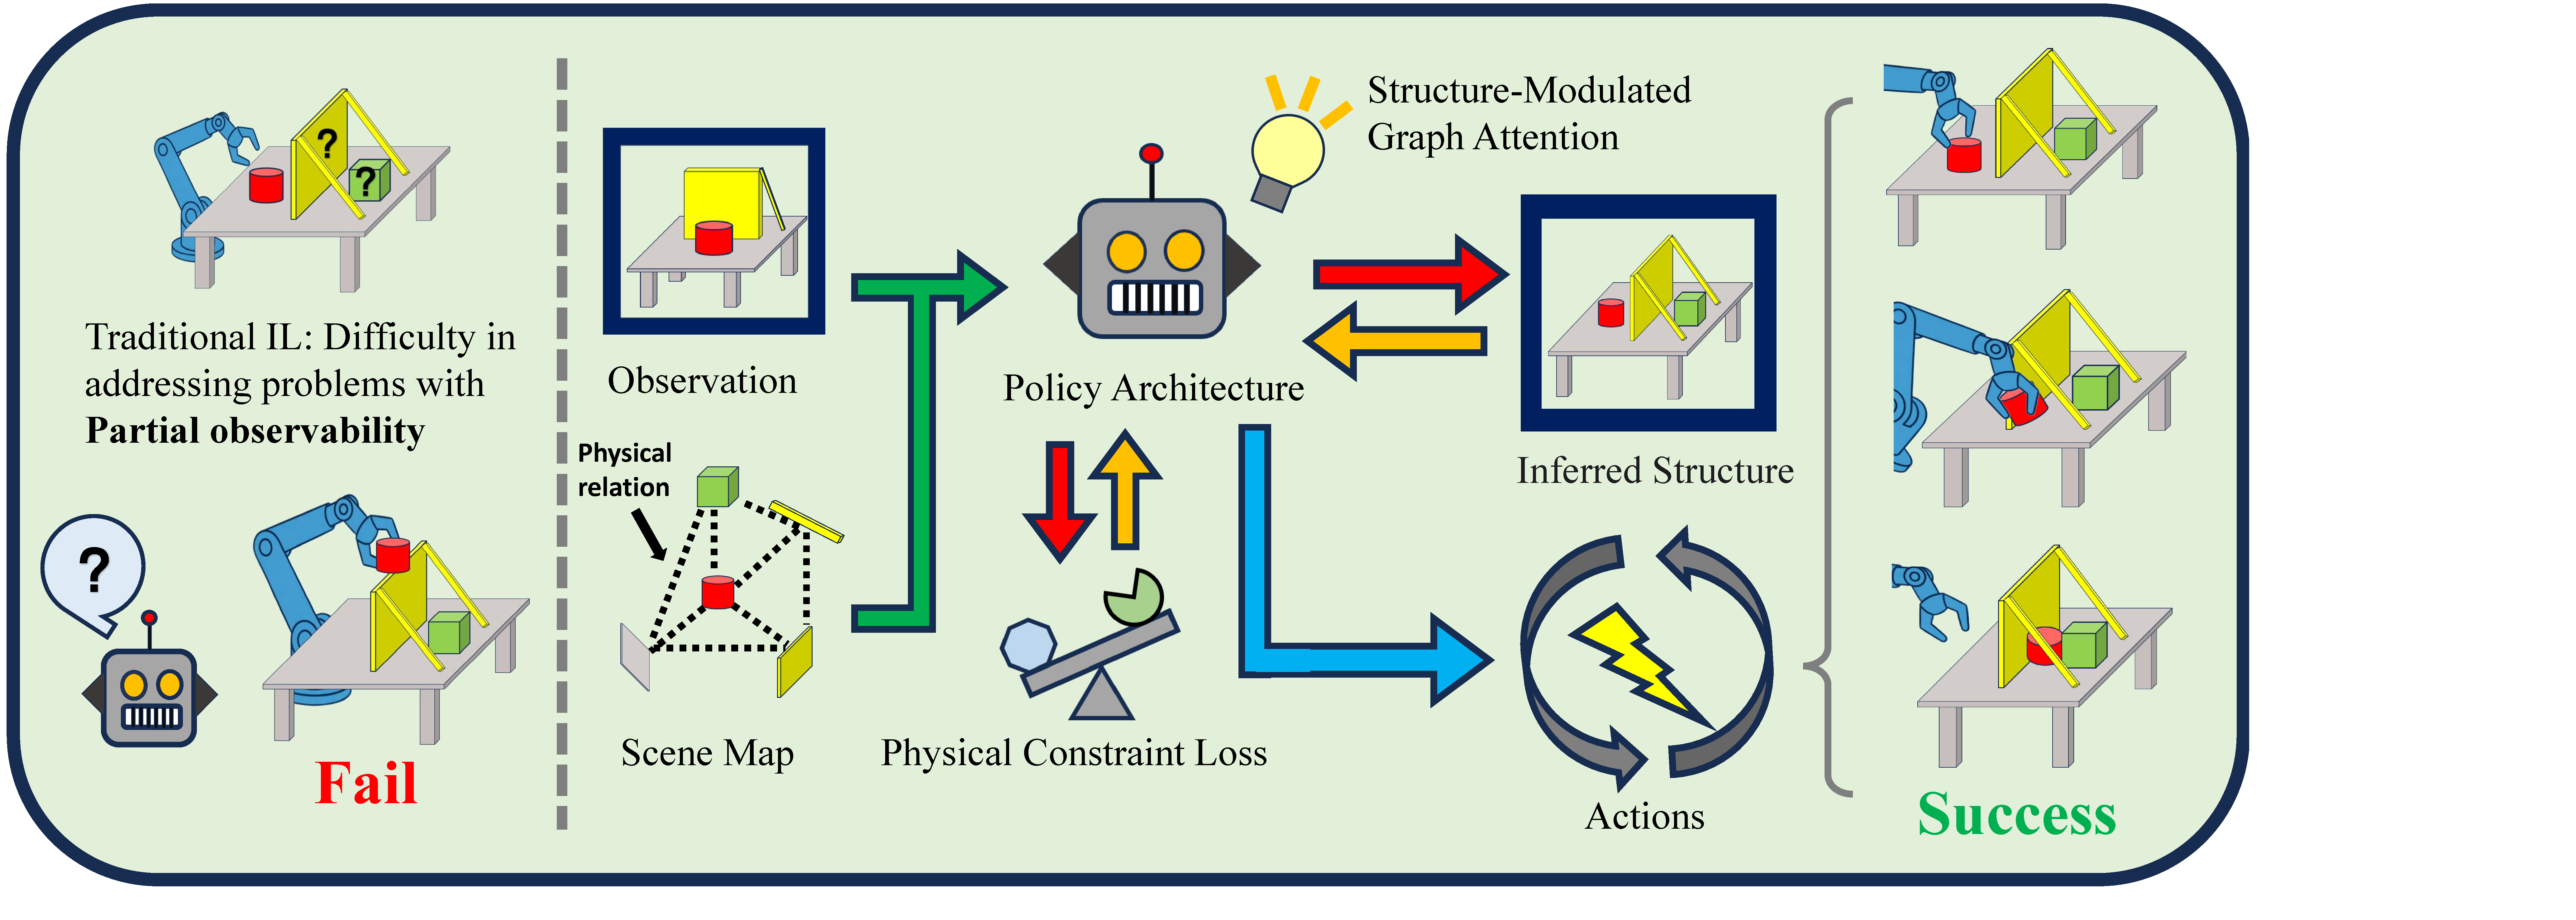
\includegraphics[width=0.85\linewidth]{figs/intro.pdf}
    \caption{Overview of MapPolicy. Traditional imitation learning can fail under partial observability because the current observation omits task-relevant structure. MapPolicy augments the observation with a Scene Map that captures physical relations, uses structure-modulated graph attention to infer hidden structure, and regularizes learned features with physical constraint loss for action prediction.}
    \label{fig:intro}
\end{figure}

Humans are often more robust in similar situations because they use prior knowledge of object structure and physical relations to infer what is not visible.
For example, when placing an object onto a shelf, a person does not need to see every layer of the shelf to infer the existence and approximate position of supporting surfaces.
This observation suggests that robust manipulation under partial observability requires more than stronger encoding of visible pixels or point clouds.
It requires a representation that exposes object structure and physical relations as explicit priors, consistent with the view that affordance and action are grounded in environmental structure~\cite{Gibson1979TheEA}.

To this end, we propose Scene Map, a structured scene representation for policy learning.
Scene Map represents a manipulation scene as a graph of geometric primitives and physical relations.
Nodes describe primitive-level object parts such as cuboids and cylinders through their shape, scale, 3D position, and rotation, while edges encode connectivity and physical constraints between primitives.
This design follows work on hierarchical graphs, part decompositions, and compositional geometric primitives~\cite{Mo2019StructureNet,Tulsiani2016LearningSA,Zou20173DPRNNGS,Paschalidou2019SuperquadricsRL,Paschalidou2020LearningUH,Sun2025ConceptFactory}.
By organizing object shape, part structure, spatial layout, and constraints in a graph, Scene Map provides structural cues that are not reliably available from the current observation alone.

Building on Scene Map, we introduce MapPolicy, an imitation learning framework that fuses map features with visual and robot state features for action prediction.
MapPolicy uses Structure-Modulated Graph Attention to propagate global structural and spatial information through primitive features, allowing visible parts and physical relations to inform the representation of hidden components.
It also uses Physical Constraint Loss to regularize learned map features with geometric and kinematic consistency.
Together, these components help the policy infer task-relevant structure from partial observations and use the inferred structure for manipulation.

We evaluate MapPolicy on 49 simulation tasks across MetaWorld, RLBench, and ManiSkill, together with five real-world tasks.
Across these settings, MapPolicy consistently improves over visual, diffusion-based, and 3D policy baselines on articulated interaction, contact-rich control, and precise spatial arrangement.

Our contributions can be summarized as follows:
\textbf{(1)} We tackle partial observability by introducing Scene Map as a structural scaffold that models object shape, part structure, spatial layout, and physical constraints.
By turning occluded but task-relevant structure into prediction targets and constraining these predictions with physical relations, Scene Map provides the policy with cues for inferring unseen components from partial observations.
\textbf{(2)} We propose MapPolicy, a policy framework that incorporates Scene Map into imitation learning by integrating structured scene representations with visual and robot state observations.
\textbf{(3)} We design two mechanisms that make structural priors effective for policy learning: Structure-Modulated Graph Attention for propagating global structural and spatial information through primitive features, and Physical Constraint Loss for enforcing geometric and kinematic consistency in learned map features.
\textbf{(4)} We conduct comprehensive evaluations across 49 simulation tasks in MetaWorld, RLBench, and ManiSkill, together with five real-world tasks, demonstrating consistent performance gains in partial-observability, articulated-interaction, contact-rich manipulation, and precise spatial-arrangement settings.


\section{Related Works}
\label{sec:related_works}

\paragraph{Imitation Learning for Robot Manipulation}
Imitation Learning (IL) provides an efficient paradigm for robot manipulation by learning a mapping function from observations to actions from demonstrations. Classical approaches are closely related to inverse reinforcement learning~\cite{Ng2000Algorithms,Abbeel2004Apprenticeship}. Modern behavior cloning trains policies with supervised objectives~\cite{Schaal1996Learning,Schaal2003Learning,Ross2010Reduction,ijcai2019Recent,Chen2023Sequential}. Multi-task and generalist manipulation policies, such as PerAct~\cite{shridhar2022peract}, CLIPort~\cite{Shridhar2022CLIPort}, Lift3D~\cite{Jia_2025_CVPR}, Baku~\cite{Haldar2025BAKU}, Track2Act~\cite{Bharadhwaj2024Track2Act}, Gen2Act~\cite{Bharadhwaj25a2025Gen2Act}, RoboAgent~\cite{Bharadhwaj2024RoboAgent}, and large-scale robot learning models~\cite{Neill2024Open}, demonstrate the benefit of stronger perception backbones, larger corpora, and more expressive policy parameterizations.

Recent generative IL methods enhance generalization and robustness.
OSVI-WM~\cite{goswami2026osviwm} introduced an end-to-end imitation learning architecture trained solely on in-domain data without large-scale pretraining and a world-model-guided trajectory generation module tailored for unseen tasks.
Latent Policy Barrier~\cite{sun2026latent} implicitly treats the latent expert demonstration distribution itself as a barrier that separates safe, in-distribution states from unsafe, out-of-distribution regions.
3D Equivariant Visuomotor Policy~\cite{hu2026d} introduces an SO(3)-equivariant policy learning framework that uses spherical projection from 2D RGB inputs to model 3D symmetries. 
% Despite these advances, most IL policies depend on currently visible observations, requiring the policy network to implicitly infer hidden object relations.
% To solve this, MapPolicy replaces implicit visual inference with an explicit Scene Map that structurally encodes both visible and occluded task components.

\paragraph{Object-Centric Representations for Manipulation}

Object-centric representations have been widely explored as a way to improve generalization in robot manipulation. Early methods use object poses, bounding boxes, or graph-structured object abstractions to decouple manipulation policies from raw pixels~\cite{Sieb2020Graph,Wang2019Deep,Devin2018Deep,Tremblay2018Deep,Tyree20226Dof,Migimatsu2020Object}. A broader object-centric learning literature studies how to discover or refine object slots, keypoints, and structured object latents from visual data~\cite{Kipf2019ContrastiveLO,Greff2019MultiObjectRL,Engelcke2019GENESISGS,Kulkarni2019UnsupervisedLO,Locatello2020Object,Qian2022Discovering,Yuan2022Sornet,Bruno2023Unsupervised,Chang2022Object,Fan2023Unsupervised,Seitzer2023Bridging}. More recent works leverage learned, foundation-model, or pretrained object-centric features to construct stronger scene encoders for manipulation, including object proposal priors~\cite{zhu2022viola}, object-centric 3D policy representations~\cite{zhu2023learning}, 3D semantic fields~\cite{Wang2025GenDP}, grounded spatial value maps~\cite{Yang2025GravMAD}, pretrained object-centric scene encoders~\cite{Qian2024SOFT}, composed ``what'' and ``where'' object representations~\cite{Shi2024Composing}, and task-oriented hierarchical object decomposition~\cite{Qian2024Task}. These methods improve the policy's ability to localize task-relevant entities and reduce reliance on global image appearance.


Despite their effectiveness, these methods primarily improve the representation or learning of the observed part of the scene. In contrast, our approach equips the policy with the ability to reason about unseen structure, addressing partial observability from a more fundamental perspective.


\section{Method}
\label{sec:method}

\subsection{Method Overview}
\label{sec:method_overview}

MapPolicy is a structured imitation learning framework that incorporates an explicit Scene Map.
At each time step, the system first constructs a scene graph from the current RGB-D observation, then encodes the graph into compact map features, and finally fuses these features with visual evidence and robot state for action prediction. In compact form, $\mathcal{G}_t = F_{\mathrm{ctor}}(I_t, D_t)$, $\mathbf{z}_{map} = F_{\mathrm{enc}}(\mathcal{G}_t)$, and $\hat{a}_t = \pi_\theta(\mathbf{z}_{map}, \mathbf{z}_{vis}, \mathbf{z}_{state})$, where $I_t$ and $D_t$ denote RGB and depth observations, $\mathbf{z}_{vis}=F_{\mathrm{vis}}(I_t)$ is the visual feature, and $\mathbf{z}_{state}=F_{\mathrm{state}}(s_t)$ is the robot state feature.

Figure~\ref{fig:pipeline} summarizes the full pipeline.
\textit{Map Constructor} instantiates Scene Map from sensor observations, \textit{Map Encoder} turns the graph into relation-aware map features, and the \textit{Policy Backbone} combines these features with visual and proprioceptive features to predict actions.
This decomposition makes the role of Scene Map explicit: it is not an external annotation consumed only during training, but the intermediate representation through which the policy reasons about scene organization under partial observability.

\begin{figure}[t]
    \centering
    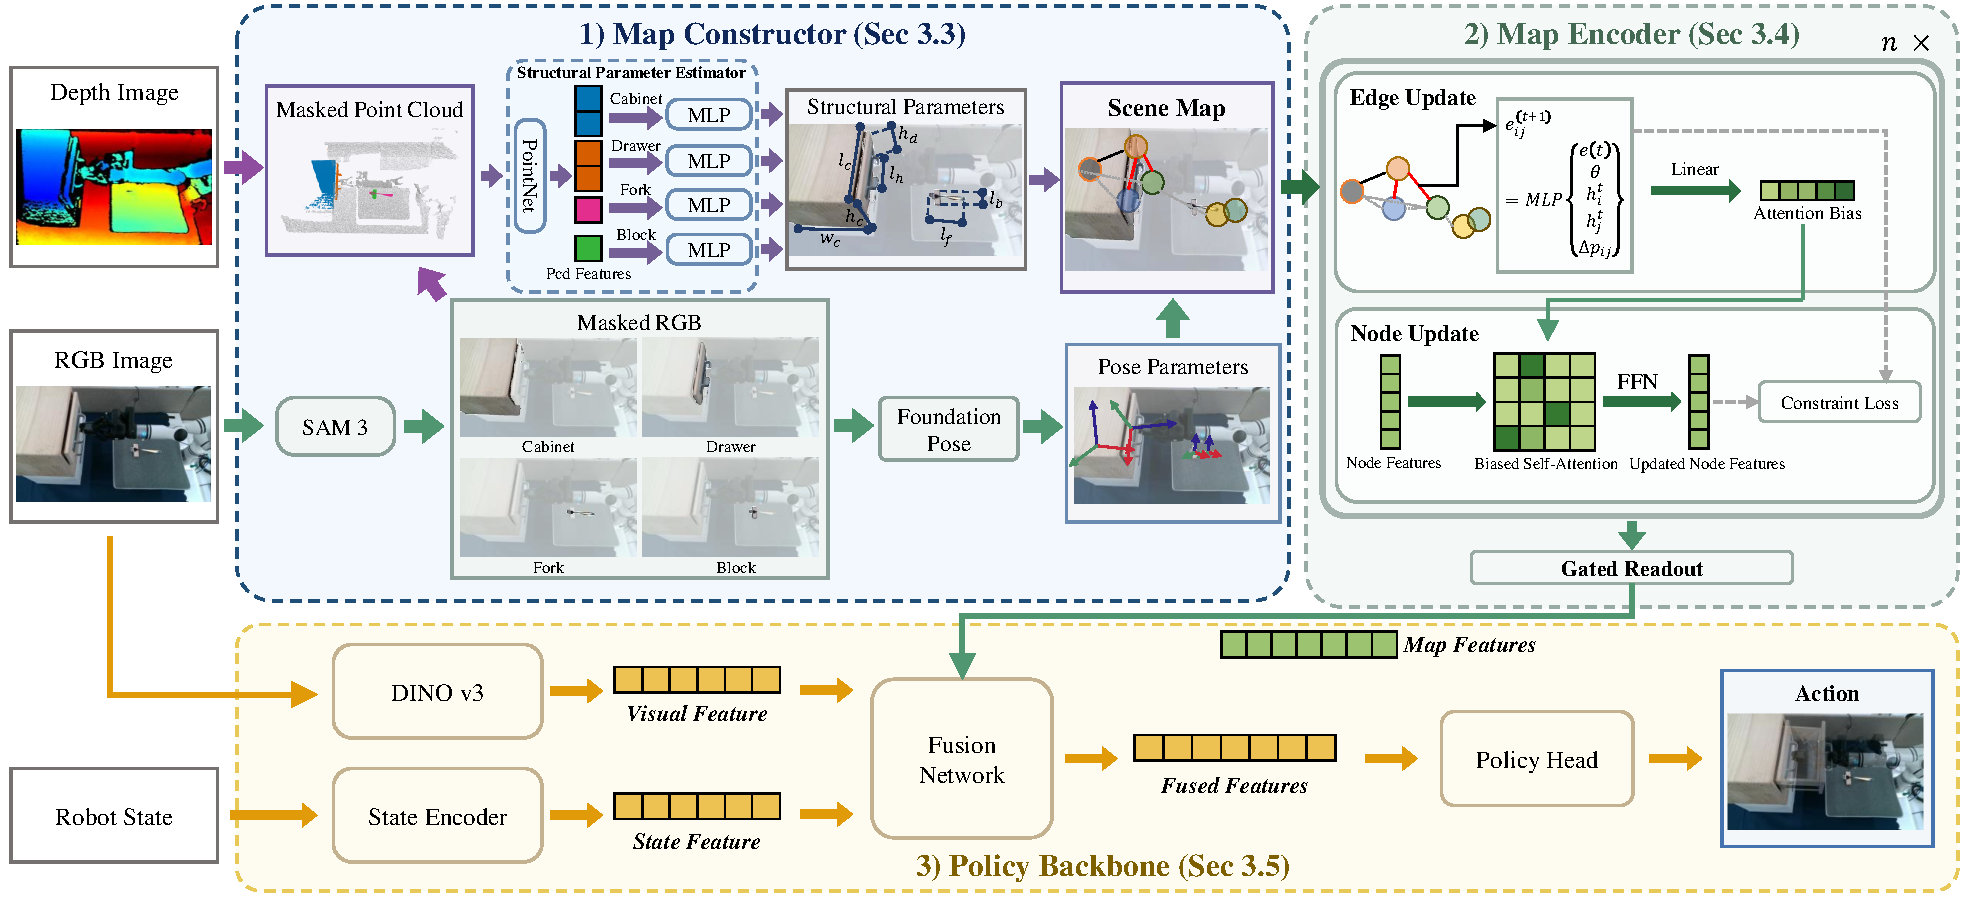
\includegraphics[width=0.95\linewidth]{figs/Pipeline.pdf}
    \caption{Overall pipeline of MapPolicy. The Map Constructor instantiates a Scene Map from RGB-D observations, the Map Encoder transforms the graph into map features, and the Policy Backbone fuses these features with visual and robot state information for action prediction.}
    \label{fig:pipeline}
\end{figure}

\subsection{Scene Map}
\label{sec:method_scene_map}

As shown in fig.~\ref{fig:scenemap}, Scene Map is a structured representation. It represents a manipulation scene as a graph $\mathcal{G}=(\mathcal{V},\mathcal{E})$. Each object is represented as an object-level subgraph, and the full scene map is obtained by composing these subgraphs together with cross-object relations. In the Scene Map example in fig.~\ref{fig:scenemap}, object parts are decomposed into primitives, and their connectivity forms a graph that preserves object structure and spatial layout even when some parts are not directly visible.

The nodes in Scene Map correspond to geometric primitives, including cuboids, cylinders, spheres, and rings as illustrated in fig.~\ref{fig:scenemap}. A node stores the primitive pose, shape or scale parameters, semantic identity, and affordance-related geometry. In compact form, we write a node as $v_i=\langle \mathbf{p}_i,\mathbf{r}_i,X_i^{pos},s_i,X_i^{aff}\rangle$, where $X_i^{pos}$ samples the primitive geometry and $X_i^{aff}$ samples manipulation-relevant regions. This primitive-level decomposition preserves object shape and part layout without collapsing them into a single object descriptor.

The edges in Scene Map represent physical constraints between primitives. Each edge is written as $e_{ij}=\langle c_{ij},\theta_{ij},a_{ij},T_{ij}\rangle$, where $c_{ij}$ is the constraint type, $\theta_{ij}$ contains continuous relation parameters, $a_{ij}$ selects the geometric anchors used by the relation, and $T_{ij}$ is the relative pose. These constraints are derived from the local geometry of primitives. For example, face anchors provide contact planes and normal directions, while axis anchors provide center lines and axial directions. The right part of fig.~\ref{fig:scenemap} describes the allowed motion of primitive B relative to primitive A, where red crosses denote forbidden translation or rotation and green arrows denote free degrees of freedom. For example, a cylindrical constraint is defined between two axis anchors: it enforces the two axes to be coaxial by constraining their direction mismatch and radial offset, while leaving translation along the axis and rotation around the axis unconstrained. Detailed primitive definitions and all six constraint types are provided in Appendix~\ref{app:scene_map_constraint}.

\begin{figure}[t]
    \centering
    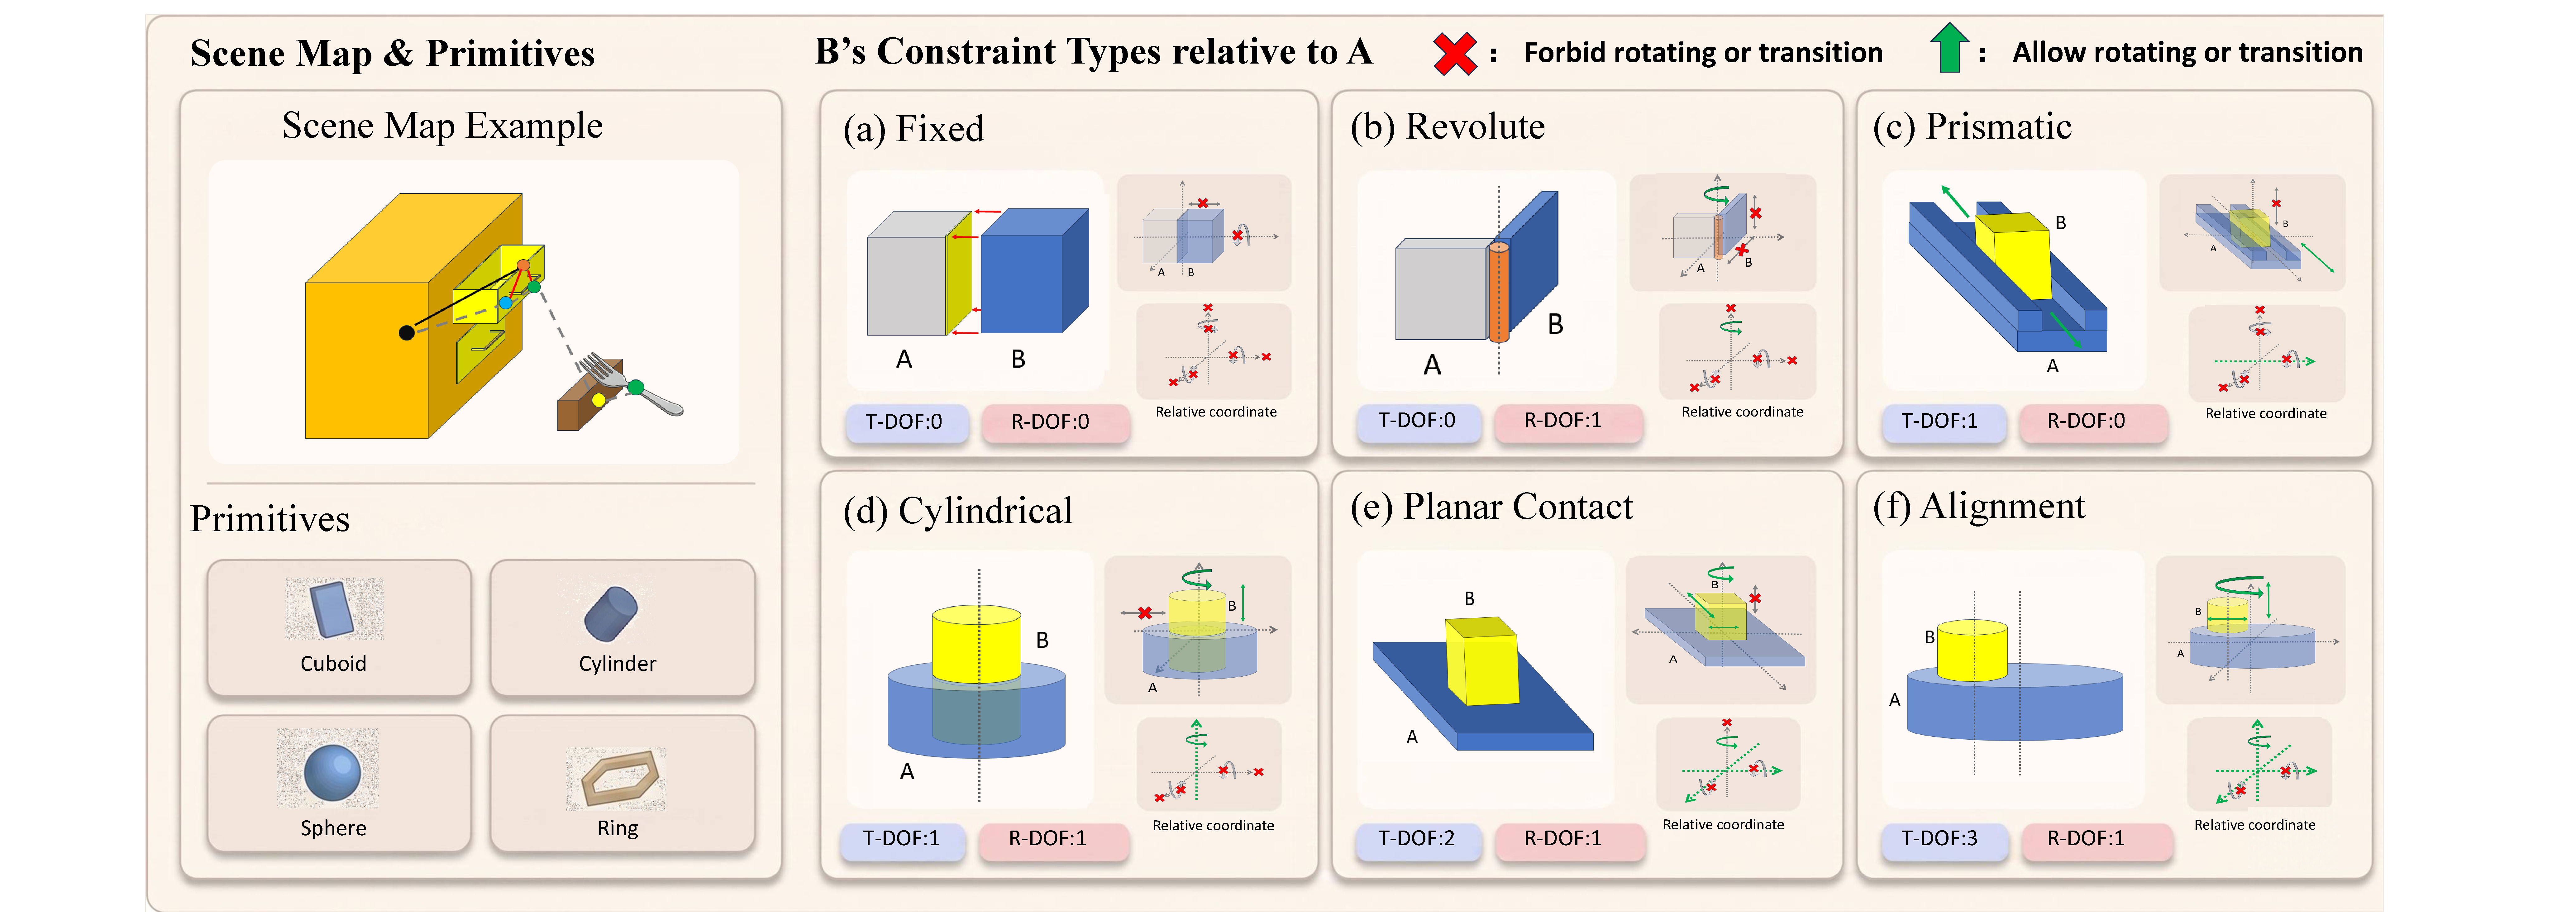
\includegraphics[width=0.95\linewidth]{figs/scenemap.pdf}
    \caption{Scene Map. The left panel shows a scene-map example and the primitive set used to decompose object structure, including cuboid, cylinder, sphere, and ring. The right panel summarizes the motion of object B relative to object A under six physical constraint types, where red crosses indicate forbidden translation or rotation and green arrows indicate allowed degrees of freedom.}
    \label{fig:scenemap}
\end{figure}

\subsection{Map Constructor}
\label{sec:map_constructor}

% As shown in fig.~\ref{fig:pipeline}(1), Map Constructor is the first module in the pipeline. Its role is to convert the current observation into an instantiated Scene Map, $\mathcal{G}_t = F_{\mathrm{ctor}}(I_t, D_t)$.

Scene Map defines \emph{what} structural information should be represented, while the constructor defines \emph{how} that information is instantiated from the current scene. Following the pipeline in fig.~\ref{fig:pipeline}, the observation is first organized into object-level evidence, including object geometry and pose estimates.

Firstly, SAM 3~\cite{sam3} is used to segment foreground objects from the RGB image, and FoundationPose~\cite{foundationposewen2024, bundlesdfwen2023} is then applied to estimate their pose parameters. In parallel, the depth image and object masks are projected into masked point clouds. A structural parameter estimator, implemented with PointNet~\cite{Qi2017PointNet} followed by separate MLP heads, encodes these point clouds and predicts the structural parameters. Finally, the estimated pose and structural parameters are combined to instantiate the Scene Map.


\subsection{Map Encoder}
\label{sec:map_encoder}

As shown in fig.~\ref{fig:pipeline}(2), Map Encoder transforms the instantiated Scene Map into compact map features $\mathbf{z}_{map} = F_{\mathrm{enc}}(\mathcal{G}_t)$ for control.
The encoder keeps node and edge streams separate at the input stage. For each node, primitive geometry, affordance samples, and semantic descriptors are embedded separately and fused into the initial node embedding $\mathbf{h}_i^0$. For each edge, relation type, continuous relation parameters, anchor descriptors, and relative pose are embedded and fused into the initial relation embedding $\mathbf{e}_{ij}^0$. This preserves both part-level attributes and explicit relation attributes before message passing.

For batched graph attention, the sparse Scene Map is packed into fixed-size node and edge tensors, $\mathbf{H}^0 \in \mathbb{R}^{B \times N \times d}$ and $\mathbf{E}^0 \in \mathbb{R}^{B \times N \times N \times d}$, where valid edge entries carry the relation attributes recovered by the constructor.
We apply a stack of Graphormer-style layers on these tensors, adapted from graph transformer mechanisms~\cite{Surveygraphtransformer, graphormer, rampasek2022GPS}. In each layer, each relation embedding is updated from its previous state and the two endpoint node states. The updated relation is then projected into a head-specific additive attention bias, which modulates node self-attention:
\begin{equation}
b_{ij,r}^{\ell} = \mathbf{w}_{b,r}^\top \mathbf{e}_{ij}^{\ell}, \qquad
\alpha_{ij,r}^{\ell} = \operatorname{softmax}_j\!\left(
\frac{(\mathbf{q}_{i,r}^{\ell})^\top \mathbf{k}_{j,r}^{\ell}}{\sqrt{d_h}} + b_{ij,r}^{\ell}
\right),
\end{equation}
where $r$ indexes attention heads. Node features are updated by the biased multi-head attention block followed by a feed-forward block with residual connections. Consequently, information can propagate between parts according to both node content and the explicit relation connecting them.
After the final layer, a gated readout computes attention weights over node states and sums them into $\mathbf{z}_{map}$. The resulting map feature is compact enough to fuse with visual and robot state features, while still being produced through edge-conditioned reasoning over the explicit Scene Map structure.

\subsection{Policy Backbone}
\label{sec:policy_backbone}

As shown in fig.~\ref{fig:pipeline}(3), Policy Backbone predicts actions from the fused multimodal representation. In parallel with map encoding, a visual encoder extracts $\mathbf{z}_{vis}$ from the current RGB observation, and a state encoder extracts $\mathbf{z}_{state}$ from proprioceptive input. The map feature, visual feature, and robot state feature are separately projected into modality tokens, fused by self-attention, and passed to an MLP policy head to predict $\hat{a}_t$.
The three branches play complementary roles. The visual branch captures currently visible evidence, the map branch provides structural priors and relation-aware context, and the state branch provides the robot's internal configuration. The policy backbone does not reconstruct scene structure again. It consumes the map features produced by the Map Encoder and turns the fused representation into a manipulation action.

\subsection{Loss Functions and Implementation Details}
\label{sec:loss_functions}
\label{sec:implementation_details}

MapPolicy uses losses at both stages of training. For Map Constructor training, the objective is $\mathcal{L}_{ctor}=\mathcal{L}_{pcd}+\lambda_{struct}\mathcal{L}_{struct}$. Here $\mathcal{L}_{pcd}$ compares the point cloud rendered from the predicted Scene Map and projected into the camera frame with the observed masked point cloud, while $\mathcal{L}_{struct}$ is a mean-squared error on structural parameters. This supervision encourages the constructed Scene Map to be both geometrically consistent with RGB-D observations and structurally aligned with the task-specific map template.

For policy training, the objective is $\mathcal{L}_{policy}=\mathcal{L}_{act}+\lambda_{phys}\mathcal{L}_{phys}$. The action loss $\mathcal{L}_{act}$ is the imitation loss on expert actions. The physical constraint loss $\mathcal{L}_{phys}$ regularizes map features by decoding edge-conditioned representations into anchor states and penalizing violations of the corresponding geometric or kinematic constraints. Detailed constraint residuals are provided in Appendix~\ref{app:scene_map_constraint}.

MapPolicy is trained in two stages. We first train the structural parameter estimator in the Map Constructor, and then freeze the constructor while training the Map Encoder and Policy Backbone. At inference time, the system follows the same observation-to-map-to-action pipeline: RGB-D observations provide object masks, poses, and masked point clouds, which instantiate a Scene Map that is encoded and fused with visual and robot state features for action prediction. The policy backbone uses a linear state encoder, attention-based multimodal fusion, and an MLP policy head. Full implementation details are provided in Appendix~\ref{app:implementation_details}.


\section{Experiments}
\label{sec:experiments}

This section evaluates whether Scene Map improves downstream manipulation policy learning beyond raw visual or geometric input. We first report main results on simulation benchmarks in sec.~\ref{sec:main_experiments}, then evaluate sim-to-real transfer in sec.~\ref{sec:real_world_experiments}. We further analyze Scene Map construction bottlenecks in sec.~\ref{sec:system_breakdown} and validate key design choices through ablations in sec.~\ref{sec:ablation_studies}.

\begin{figure}[t]
    \centering
    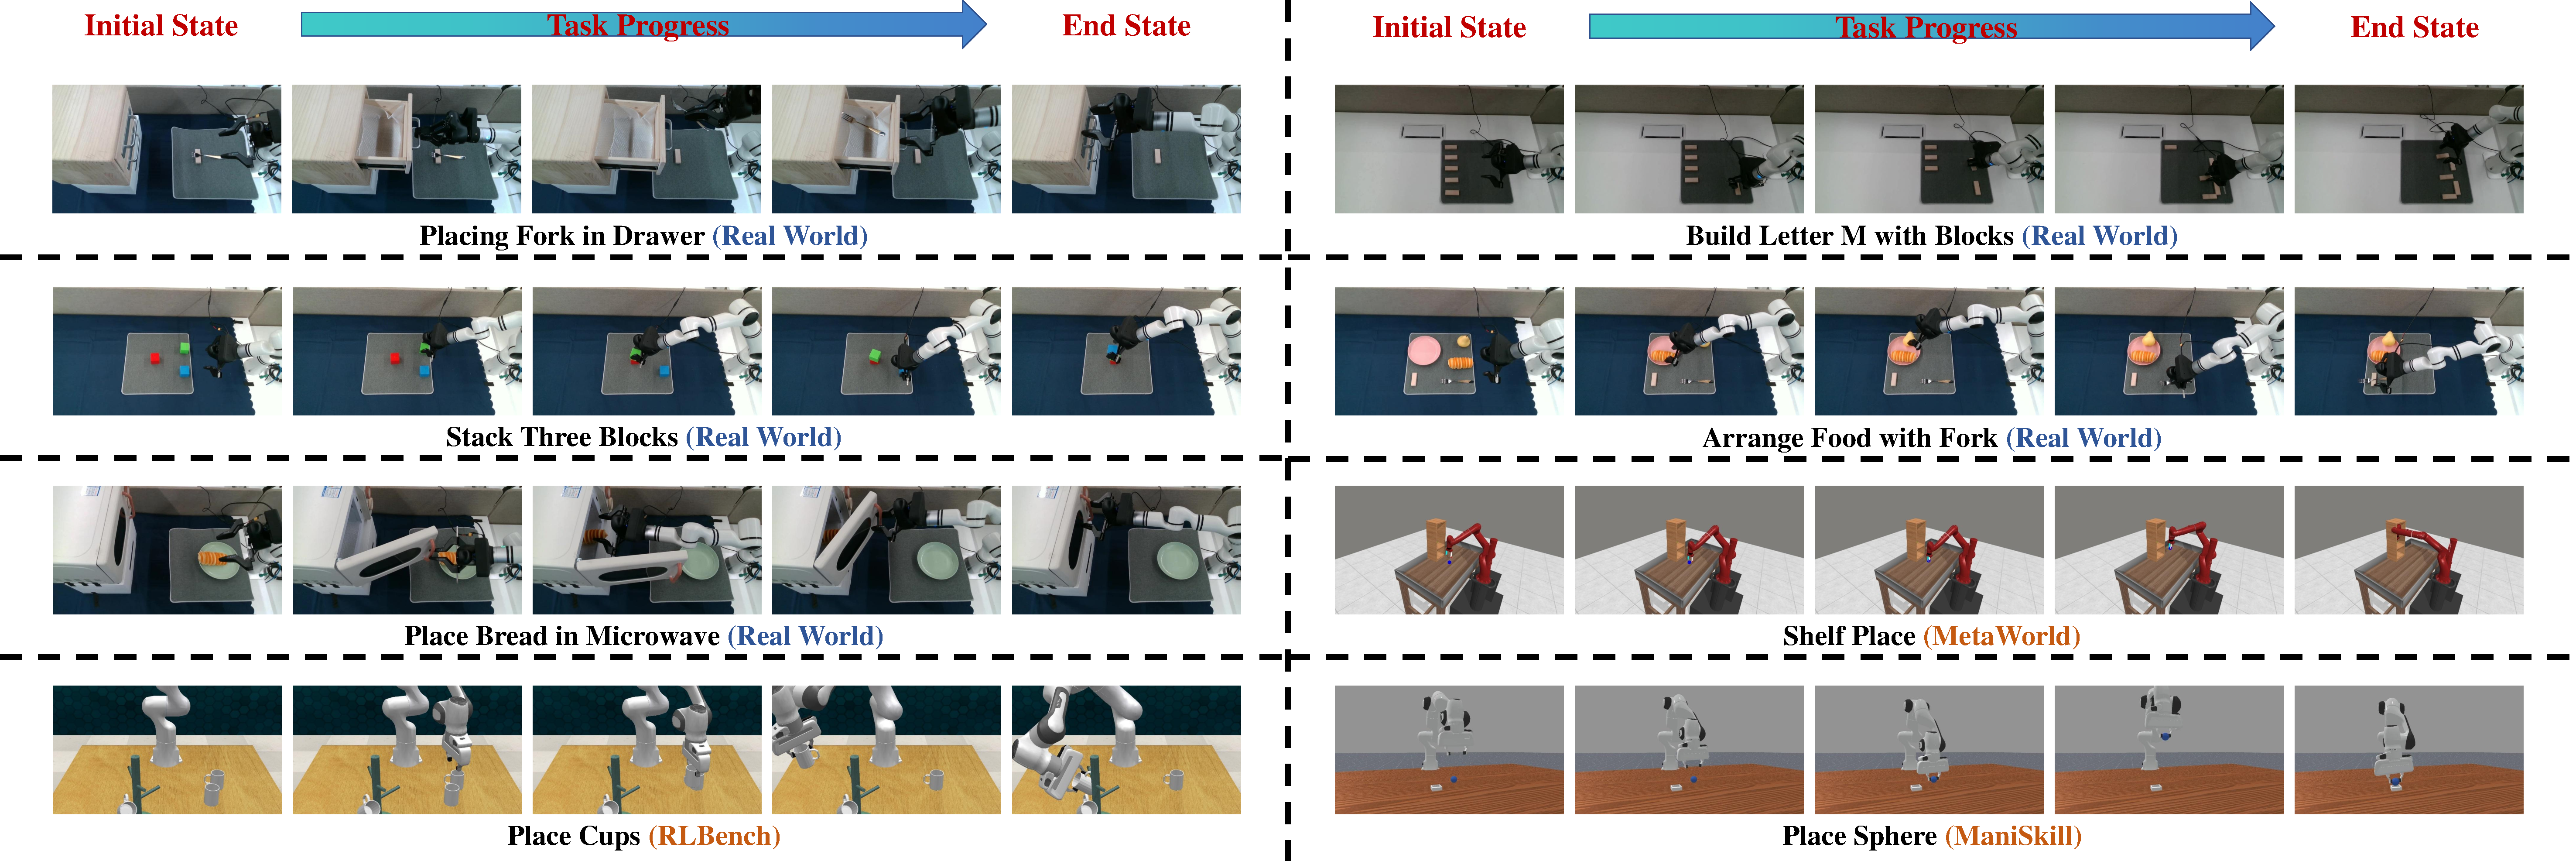
\includegraphics[width=0.95\linewidth]{figs/demonstration.pdf}
    \caption{Demonstrations of the evaluation tasks. The figure shows all five real-world tasks and representative tasks from MetaWorld~\cite{Yu2020Meta,mclean2025metaworld}, RLBench~\cite{James2020RLBench}, and ManiSkill~\cite{Gu2023ManiSkill2}, illustrating the diversity of articulated interaction, object arrangement, and geometrically constrained manipulation considered in our experiments.}
    \label{fig:demonstration}
\end{figure}

\subsection{Main Experiments in Simulation Benchmarks}
\label{sec:main_experiments}

We evaluate MapPolicy on three simulation benchmarks with complementary characteristics: MetaWorld~\cite{Yu2020Meta,mclean2025metaworld}, RLBench~\cite{James2020RLBench}, and ManiSkill~\cite{Gu2023ManiSkill2}. Together, they cover classical single-task manipulation, large-scale multi-task interaction, and tabletop manipulation.

\textbf{Experiment Settings.}
We benchmark MapPolicy on three suites.
\textbf{MetaWorld}~\cite{Yu2020Meta,mclean2025metaworld} contains 25 tasks in our evaluation and is used to test whether Scene Map helps on diverse classical MuJoCo-based manipulation problems requiring part-level interaction and precise spatial reasoning~\cite{todorov2012mujoco}.
\textbf{RLBench}~\cite{James2020RLBench} contains 18 tasks in our evaluation and is used to test whether the benefits of Scene Map persist in visually richer and more diverse multi-task settings.
\textbf{ManiSkill}~\cite{Gu2023ManiSkill2} contains six tasks from the official \textit{Table-Top 2 Finger Gripper Tasks} category, including \textit{PegInsertionSide-v1}, \textit{PlaceSphere-v1}, \textit{PlugCharger-v1}, \textit{PullCubeTool-v1}, \textit{StackCube-v1}, and \textit{StackPyramid-v1}, and is used to test MapPolicy on tabletop RGB-D manipulation with strong geometric and contact constraints.
Across all three benchmarks, the main metric is task success rate. We report mean and standard deviation across five random seeds for the main simulation results. Detailed training and evaluation protocols are provided in Appendix~\ref{app:experimental_protocols}.

\textbf{Baselines.}
We compare against strong baselines from three categories: diffusion-based policies, general-purpose visuomotor foundation policies, and 3D manipulation policies.
On MetaWorld, we compare against \textit{Diffusion Policy}~\cite{chi2024diffusionpolicy}, \textit{3D Diffusion Policy}~\cite{Ze2024DP3}, \textit{$\pi_0$}~\cite{black2026pi0visionlanguageactionflowmodel}, and \textit{Lift3D}~\cite{Jia_2025_CVPR}.
On RLBench, we compare against published baselines reported in prior work, including \textit{PerAct}~\cite{shridhar2022peract}, \textit{3D Diffuser Actor}~\cite{3d_diffuser_actor}, \textit{RVT-2}~\cite{goyal2024rvt2}, and the \textit{PDFactor} family~\cite{Tian_2025_CVPR}, using their reported numbers.
On ManiSkill, we compare against \textit{Diffusion Policy}~\cite{chi2024diffusionpolicy}, \textit{3D Diffusion Policy}~\cite{Ze2024DP3}, \textit{Octo}~\cite{octo_2023}, and \textit{$\pi_0$}~\cite{black2026pi0visionlanguageactionflowmodel}.

\begin{table*}[t]
\centering
\caption{Summary of main simulation results. We report average success rate (\%) across all evaluated tasks in each benchmark. Full per-task results are provided in Appendix~\ref{app:full_sim_results}.}
\label{tab:main_results_summary}
\small
\setlength{\tabcolsep}{6pt}
\begin{adjustbox}{max width=\textwidth}
\begin{tabular}{lc|lc|lc}
\toprule
\rowcolor{tablehead}
\multicolumn{2}{c|}{MetaWorld~\cite{Yu2020Meta,mclean2025metaworld} (25 tasks)} &
\multicolumn{2}{c|}{RLBench~\cite{James2020RLBench} (18 tasks)} &
\multicolumn{2}{c}{ManiSkill~\cite{Gu2023ManiSkill2} (6 tasks)} \\
\rowcolor{tablehead}
Method & Mean S.R. (\%) & Method & Mean S.R. (\%) & Method & Mean S.R. (\%) \\
\midrule
Diffusion Policy~\cite{chi2024diffusionpolicy} & 27.3 &
PerAct~\cite{shridhar2022peract} & 49.4 &
Diffusion Policy~\cite{chi2024diffusionpolicy} & 26.8 \\
3D Diffusion Policy~\cite{Ze2024DP3} & 51.1 &
3D Diffuser Actor~\cite{3d_diffuser_actor} & 81.4 &
3D Diffusion Policy~\cite{Ze2024DP3} & 53.8 \\
$\pi_0$~\cite{black2026pi0visionlanguageactionflowmodel} & 69.5 &
RVT-2~\cite{goyal2024rvt2} & 81.4 &
Octo~\cite{octo_2023} & 16.8 \\
\underline{Lift3D~\cite{Jia_2025_CVPR}} & \underline{78.8} &
\underline{PDFactor~\cite{Tian_2025_CVPR}} & \underline{87.3} &
\underline{$\pi_0$~\cite{black2026pi0visionlanguageactionflowmodel}} & \underline{54.0} \\
\rowcolor{tablehead}
\textbf{MapPolicy} & \textbf{93.2} &
\textbf{MapPolicy} & \textbf{94.8} &
\textbf{MapPolicy} & \textbf{73.0} \\
\bottomrule
\end{tabular}
\end{adjustbox}
\end{table*}


\begin{table}[t]
\centering
\caption{Real-world results. We report success rate (\%) over 100 trials for each real-world manipulation task. Best results are in \textbf{bold}, and second best are \underline{underlined}.}
\label{tab:real_world_results}
\small
\setlength{\tabcolsep}{4pt}
\begin{adjustbox}{max width=0.85\linewidth}
\begin{tabular}{l|c|ccccc}
\toprule
\rowcolor{tablehead}
Method & Avg. &
\shortstack{Place Fork\\in Drawer} &
\shortstack{Stack Three\\Blocks} &
\shortstack{Arrange Food\\with Fork} &
\shortstack{Place Bread\\in Microwave} &
\shortstack{Build Letter M\\with Blocks} \\
\midrule
Diffusion Policy~\cite{chi2024diffusionpolicy} & 15.4 & 12 & 6 & 41 & 18 & 0 \\
3D Diffusion Policy~\cite{Ze2024DP3} & 33.6 & 38 & 21 & 66 & 43 & 0 \\
Lift3D~\cite{Jia_2025_CVPR} & 36.2 & 41 & 25 & 69 & 46 & 0 \\
$\pi_0$~\cite{black2026pi0visionlanguageactionflowmodel} & \underline{49.8} & \underline{51} & \underline{39} & \underline{83} & \underline{61} & \underline{15} \\
\midrule
MapPolicy (Ours) & \textbf{81.4} & \textbf{87} & \textbf{78} & \textbf{95} & \textbf{84} & \textbf{63} \\
\bottomrule
\end{tabular}
\end{adjustbox}
\end{table}



\textbf{Results.}
\textbf{MetaWorld}~\cite{Yu2020Meta,mclean2025metaworld} tests classical manipulation tasks requiring actionable-part identification and local spatial reasoning. As shown in tab.~\ref{tab:main_results_summary}, MapPolicy achieves 93.2\% average success rate, outperforming the strongest prior baseline Lift3D at 78.8\%. The gains are particularly meaningful on articulated interaction, contact-rich manipulation, and precise placement. Full per-task results are provided in Appendix~\ref{app:full_sim_results}.
\textbf{RLBench}~\cite{James2020RLBench} evaluates larger-scale multi-task scenes with richer visual variation and multi-object interaction. MapPolicy reaches 94.8\% average success rate, improving over the strongest published baseline PDFactor at 87.3\%, indicating that Scene Map benefits extend beyond classical manipulation settings.
\textbf{ManiSkill}~\cite{Gu2023ManiSkill2} focuses on tabletop tasks with strong geometric constraints such as insertion, plugging, stacking, and tool use. MapPolicy obtains 73.0\% average success rate, outperforming $\pi_0$ at 54.0\% and 3D Diffusion Policy at 53.8\%, with the largest gains on tasks where explicit structure is directly relevant to action success.

\subsection{Real-World Experiments}
\label{sec:real_world_experiments}

We evaluate whether the Scene Map interface transfers from simulation to real RGB-D manipulation on a Realman 75-BF robot arm with 7 DoF and a pika gripper, running at 30 Hz. RGB-D observations are captured by an NVIDIA RealSense D415, and point clouds are constructed with Open3D~\cite{Zhou2018Open3D}. We reuse representative baselines from our simulation study for the real-world setting. In the current real-robot evaluation, we directly deploy \textit{Diffusion Policy}~\cite{chi2024diffusionpolicy} and \textit{3D Diffusion Policy}~\cite{Ze2024DP3} as the primary reproducible baselines, while \textit{$\pi_0$}~\cite{black2026pi0visionlanguageactionflowmodel} and \textit{Lift3D}~\cite{Jia_2025_CVPR} provide additional reference points for method positioning. For each real-world task, we execute each method for 100 trials and report task success rate as the main metric.


\textbf{Task Suite.}
We design five real-world tasks that cover articulated interaction, reflective-object grasping, multi-object spatial reasoning, and long-horizon arrangement.
\textit{Place Fork in Drawer} consists of four stages: opening a closed drawer, picking up a fork placed on a block, placing it into the drawer, and closing the drawer. This task is challenging because it combines articulated-object manipulation with grasping a thin, irregular, and reflective metal object.
\textit{Stack Three Blocks} requires first placing a green block on a red block and then placing a blue block on the green block. The main difficulty is maintaining the correct spatial relation across three objects during sequential stacking.
\textit{Arrange Food with Fork} consists of placing bread on a plate, placing a pear on the plate, and then placing a fork on a block stand. Although this is a more common tabletop arrangement task, it still tests compositional multi-object placement in a cluttered real scene.
\textit{Place Bread in Microwave} consists of opening the microwave door, transferring bread from a plate into the microwave, and closing the door. This task emphasizes articulated manipulation under partial occlusion and changing scene geometry.
\textit{Build Letter M with Blocks} requires arranging five blocks into a specified global shape. Unlike local pick-and-place tasks, this setting tests whether the policy can reason about a target spatial pattern and adjust placements online to satisfy the final global arrangement.

\textbf{Results.}
As shown in tab.~\ref{tab:real_world_results}, we report success rate over 100 real-robot trials for each task and each method. MapPolicy transfers robustly to the real world and is particularly effective on tasks where success depends on understanding hidden structure, articulated state, or global spatial layout. Compared with Diffusion Policy~\cite{chi2024diffusionpolicy} and 3D Diffusion Policy~\cite{Ze2024DP3}, MapPolicy produces more stable multi-step behavior on drawer and microwave tasks and better preserves the required inter-object arrangement on stacking and shape-construction tasks. These results are consistent with our central claim: explicit Scene Map helps the policy maintain a manipulation-oriented representation of object structure and spatial relations even when raw observations are noisy, partially occluded, or insufficient to reveal the full scene state.

\subsection{System Error Breakdown}
\label{sec:system_breakdown}

\begin{table}[t]
\centering
\caption{System error breakdown on MetaWorld~\cite{Yu2020Meta,mclean2025metaworld}. We use oracle replacements to identify the dominant bottleneck in MapPolicy. Oracle quantities are used only for analysis and are not part of the inference interface. $\Delta$ reports the improvement over Full MapPolicy.}
\label{tab:system_breakdown}
\small
\setlength{\tabcolsep}{6pt}
\begin{adjustbox}{max width=0.9\columnwidth}
\begin{tabular}{l|ccc|>{\columncolor{white}}c|c}
\toprule
Setting & GT Extraction & GT Object Pose & GT Structural Size & Avg. Success & $\Delta$ \\
\midrule
Full MapPolicy &  &  &  & \cellcolor{blue1}93.2 & 0.0 \\
+ GT Extraction & $\checkmark$ &  &  & \cellcolor{blue1}93.4 & +0.2 \\
+ GT Object Pose &  & $\checkmark$ &  & \cellcolor{blue2}94.0 & +0.8 \\
+ GT Structural Size &  &  & $\checkmark$ & \cellcolor{blue2}94.6 & +1.4 \\
+ GT Extraction + GT Object Pose & $\checkmark$ & $\checkmark$ &  & \cellcolor{blue1}93.4 & +0.2 \\
+ GT Extraction + GT Structural Size & $\checkmark$ &  & $\checkmark$ & \cellcolor{blue3}95.1 & +1.9 \\
+ GT Object Pose + GT Structural Size &  & $\checkmark$ & $\checkmark$ & \cellcolor{blue4}95.9 & +2.7 \\
+ GT Extraction + GT Object Pose + GT Structural Size & $\checkmark$ & $\checkmark$ & $\checkmark$ & \cellcolor{blue4}96.0 & +2.8 \\
\bottomrule
\end{tabular}
\end{adjustbox}
\end{table}


\begin{table*}[t]
\centering
% --- Left table: Scene Map contents ---
\begin{minipage}[t]{0.52\textwidth}
    \centering
    \caption{Ablation study on Scene Map representation by varying node and edge attributes on MetaWorld~\cite{Yu2020Meta,mclean2025metaworld}.}
    \label{tab:ablation_map_contents}
    \scriptsize
    \resizebox{\linewidth}{!}{
        \begin{tabular}{c|cccc|cccc|c}
        \hline
         & \multicolumn{4}{c|}{Node} & \multicolumn{4}{c|}{Edge} &  \\
        \hline
         & Geo & Pose & Sem & Aff & Type & Param & Anchor & RelPose & \textbf{Mean} \\
        \hline
        Ex1 & $\checkmark$ & - & - & - & - & - & - & - & \cellcolor{blue1}\textbf{72.4} \\
        Ex2 & $\checkmark$ & $\checkmark$ & - & - & - & - & - & - & \cellcolor{blue1}\textbf{78.1} \\
        Ex3 & $\checkmark$ & $\checkmark$ & $\checkmark$ & $\checkmark$ & - & - & - & - & \cellcolor{blue2}\textbf{83.5} \\
        Ex4 & $\checkmark$ & $\checkmark$ & $\checkmark$ & $\checkmark$ & $\checkmark$ & - & - & - & \cellcolor{blue2}\textbf{86.7} \\
        Ex5 & $\checkmark$ & $\checkmark$ & $\checkmark$ & $\checkmark$ & $\checkmark$ & $\checkmark$ & - & - & \cellcolor{blue3}\textbf{88.9} \\
        Ex6 & $\checkmark$ & $\checkmark$ & $\checkmark$ & $\checkmark$ & $\checkmark$ & $\checkmark$ & $\checkmark$ & - & \cellcolor{blue3}\textbf{91.4} \\
        \textbf{\underline{Ex7}} & $\checkmark$ & $\checkmark$ & $\checkmark$ & $\checkmark$ & $\checkmark$ & $\checkmark$ & $\checkmark$ & $\checkmark$ & \cellcolor{blue4}\textbf{93.2} \\
        \hline
        \end{tabular}
    }
\end{minipage}
\hfill
% --- Right table: encoder and fusion ---
\begin{minipage}[t]{0.46\textwidth}
    \centering
    \caption{Ablation study on map encoder and multimodal fusion design choices on MetaWorld~\cite{Yu2020Meta,mclean2025metaworld}.}
    \label{tab:ablation_encoder_fusion}
    \scriptsize
    \resizebox{\linewidth}{!}{
        \begin{tabular}{c|cccc|ccc|c}
        \hline
         & \multicolumn{4}{c|}{Map Encoder} & \multicolumn{3}{c|}{Fusion} &  \\
        \hline
         & Pool & PN & Trans. & Graph & Concat & MLP & Attn & \textbf{Mean} \\
        \hline
        Ex1 & $\checkmark$ & - & - & - & - & - & $\checkmark$ & \cellcolor{blue1}\textbf{75.6} \\
        Ex2 & - & $\checkmark$ & - & - & - & - & $\checkmark$ & \cellcolor{blue2}\textbf{82.3} \\
        Ex3 & - & - & $\checkmark$ & - & - & - & $\checkmark$ & \cellcolor{blue3}\textbf{89.1} \\
        \textbf{\underline{Ex4}} & - & - & - & $\checkmark$ & - & - & $\checkmark$ & \cellcolor{blue4}\textbf{93.2} \\
        \hline
        Ex5 & - & - & - & $\checkmark$ & $\checkmark$ & - & - & \cellcolor{blue2}\textbf{84.2} \\
        Ex6 & - & - & - & $\checkmark$ & - & $\checkmark$ & - & \cellcolor{blue3}\textbf{87.6} \\
        \textbf{\underline{Ex7}} & - & - & - & $\checkmark$ & - & - & $\checkmark$ & \cellcolor{blue4}\textbf{93.2} \\
        \hline
        \end{tabular}
    }
\end{minipage}

\par
\begin{minipage}{0.98\textwidth}
    \centering
    \scriptsize
    \textit{Note:}
    Geo = part geometry, Sem = semantic identity, Aff = affordance attributes.
    Param = continuous relation parameters, RelPose = relative pose.
    PN = PointNet~\cite{Qi2017PointNet}, Trans. = Transformer, Graph = graph encoder, Attn = attention fusion.
    Darker blue indicates better performance.
\end{minipage}
\end{table*}


MapPolicy is a multi-stage system whose final performance depends not only on downstream policy learning, but also on the quality of Scene Map construction. To identify the dominant bottleneck, we perform a system error breakdown on MetaWorld~\cite{Yu2020Meta,mclean2025metaworld} using oracle replacements. Since several error sources in MapPolicy can be independently controlled, we use a combinatorial oracle analysis instead of a single sequential replacement protocol.

\textbf{Setup.}
We analyze three independent sources of structural error: object extraction, object-pose estimation, and structural-size estimation. For each source, we replace the predicted quantity with its ground-truth counterpart and evaluate the resulting average success rate. All oracle quantities in this subsection are used only for analysis and are not part of the inference interface of MapPolicy.

\textbf{Results.}
The main result is summarized in tab.~\ref{tab:system_breakdown}, formatted as a 2D oracle matrix. The table contains three oracle columns, \textit{GT Extraction}, \textit{GT Object Pose}, and \textit{GT Structural Size}, together with one performance column, \textit{Avg. Success}. The rows enumerate all combinations of the three oracle sources.
This analysis should be read in two stages. First, the single-factor replacements reveal which structural error source is the dominant independent bottleneck. Second, the joint replacements reveal whether different error sources interact strongly or contribute largely independent errors. This subsection therefore identifies which part of the MapPolicy pipeline deserves the highest priority for improvement.


\subsection{Ablation Studies}
\label{sec:ablation_studies}



\begin{table*}[t]
\centering
\caption{Ablation study on training losses on MetaWorld~\cite{Yu2020Meta,mclean2025metaworld}. Map Attr. GT supervises the scene-dependent node and edge attributes used to instantiate Scene Map, Chamfer supervises map-induced point-cloud geometry, and Physical enforces relation-specific constraints.}
\label{tab:ablation_loss_presence}
\scriptsize
\setlength{\tabcolsep}{4pt}
\begin{adjustbox}{max width=\textwidth}
\begin{tabular}{c|cccc|c@{\hspace{12pt}}c|cccc|c}
\toprule
 & \multicolumn{4}{c|}{Loss Terms} &  &  & \multicolumn{4}{c|}{Loss Terms} &  \\
\cmidrule(lr){2-5} \cmidrule(lr){8-11}
Setting & Action & Map Attr. GT & Chamfer & Physical & Avg. Success &
Setting & Action & Map Attr. GT & Chamfer & Physical & Avg. Success \\
\midrule
Ex1 & $\checkmark$ & - & - & - & \cellcolor{blue1}80.6 &
Ex5 & $\checkmark$ & $\checkmark$ & $\checkmark$ & - & \cellcolor{blue2}88.7 \\
Ex2 & $\checkmark$ & $\checkmark$ & - & - & \cellcolor{blue1}83.4 &
Ex6 & $\checkmark$ & $\checkmark$ & - & $\checkmark$ & \cellcolor{blue3}89.5 \\
Ex3 & $\checkmark$ & - & $\checkmark$ & - & \cellcolor{blue2}84.1 &
Ex7 & $\checkmark$ & - & $\checkmark$ & $\checkmark$ & \cellcolor{blue4}\underline{92.4} \\
Ex4 & $\checkmark$ & - & - & $\checkmark$ & \cellcolor{blue1}82.8 &
\textbf{\underline{Ex8}} & $\checkmark$ & $\checkmark$ & $\checkmark$ & $\checkmark$ & \cellcolor{blue4}\textbf{93.2} \\
\bottomrule
\end{tabular}
\end{adjustbox}
\end{table*}


We design ablations to answer three questions: whether explicit Scene Map is necessary as a representation, how Scene Map should be encoded and fused with visual information, and which supervision terms make the learned map most useful for downstream control.

\textbf{Scene Map Representation.}
We first evaluate which contents inside Scene Map are most important for policy learning. We conduct this ablation on MetaWorld~\cite{Yu2020Meta,mclean2025metaworld} and keep the policy backbone and training recipe fixed, changing only the attributes included in the map representation. Table~\ref{tab:ablation_map_contents} progressively adds node attributes, including part geometry, pose, semantic identity, and affordance-related information, and then edge attributes, including relation type, continuous relation parameters, anchor references, and relative pose. This comparison separates the contribution of part-level node descriptors from the contribution of explicit cross-part relations. If edge attributes provide additional gains beyond node-only representations, the conclusion is that Scene Map helps not only by describing object parts, but also by modeling the structural and physical relations among them.



\textbf{Structure-Aware Encoder and Fusion.}
Given a Scene Map, the next question is how it should be encoded and fused with visual information. We therefore study both the choice of map encoder and the choice of fusion strategy. Table~\ref{tab:ablation_encoder_fusion} compares four encoders while keeping the Scene Map representation fixed: \textit{Pooling}, \textit{PointNet}~\cite{Qi2017PointNet}, \textit{Transformer}~\cite{Kim2021Transformer}, and \textit{Graph Encoder}. This comparison tests whether relation-aware graph encoding is necessary to fully exploit the node-edge structure of Scene Map. We then fix the best map encoder and compare three fusion strategies: \textit{Concat}, \textit{MLP fusion}, and \textit{Attention fusion}. These results show whether the information in Scene Map can be effectively used by naive concatenation or whether a stronger fusion mechanism is needed to integrate structural and visual cues for downstream action prediction.

\textbf{Loss Design.}
We keep action imitation enabled and ablate three auxiliary losses: map-attribute supervision, point-cloud Chamfer supervision, and physical constraint regularization. Table~\ref{tab:ablation_loss_presence} shows that each auxiliary loss improves over action imitation alone, while combining Chamfer supervision with physical constraints gives the strongest partial combination and using all three losses achieves the best performance.



\section{Conclusion}

We studied robot manipulation under partial observability and argued that the core challenge is missing task-relevant structure rather than missing visual evidence alone. We introduced Scene Map, a graph representation of object shape, part structure, spatial layout, and physical constraints, and proposed MapPolicy to fuse map, visual, and robot state features for imitation learning. Across 49 simulation tasks in MetaWorld, RLBench, and ManiSkill, together with five real-world tasks, MapPolicy consistently improves over strong baselines on partial observability, articulated interaction, contact-rich manipulation, and precise spatial arrangement. These results suggest that explicit structural priors can improve manipulation policy learning beyond raw visual input or unstructured geometry alone. Future work should improve the robustness and generality of Scene Map construction for more open-ended real-world environments.


\newpage

\bibliographystyle{plainnat} 
\bibliography{references}

% \section*{References}


% References follow the acknowledgments in the camera-ready paper. Use unnumbered first-level heading for
% the references. Any choice of citation style is acceptable as long as you are
% consistent. It is permissible to reduce the font size to \verb+small+ (9 point)
% when listing the references.
% Note that the Reference section does not count towards the page limit.
% \medskip


% {
% \small


% [1] Alexander, J.A.\ \& Mozer, M.C.\ (1995) Template-based algorithms for
% connectionist rule extraction. In G.\ Tesauro, D.S.\ Touretzky and T.K.\ Leen
% (eds.), {\it Advances in Neural Information Processing Systems 7},
% pp.\ 609--616. Cambridge, MA: MIT Press.


% [2] Bower, J.M.\ \& Beeman, D.\ (1995) {\it The Book of GENESIS: Exploring
%   Realistic Neural Models with the GEneral NEural SImulation System.}  New York:
% TELOS/Springer--Verlag.


% [3] Hasselmo, M.E., Schnell, E.\ \& Barkai, E.\ (1995) Dynamics of learning and
% recall at excitatory recurrent synapses and cholinergic modula    tion in rat
% hippocampal region CA3. {\it Journal of Neuroscience} {\bf 15}(7):5249-5262.
% }


%%%%%%%%%%%%%%%%%%%%%%%%%%%%%%%%%%%%%%%%%%%%%%%%%%%%%%%%%%%%

\newpage
\appendix

\section{Technical appendices and supplementary material}
\paragraph{Appendix organization.}
This appendix follows the order of the main paper. Appendix~\ref{app:scene_map_constraint} details the Scene Map representation and physical constraint loss used in sec.~\ref{sec:method_scene_map} and sec.~\ref{sec:loss_functions}. Appendix~\ref{app:complexity} discusses computational complexity, Appendix~\ref{app:mappolicy_procedure} summarizes the full MapPolicy procedure, and Appendix~\ref{app:implementation_details} provides implementation details for the method. Appendix~\ref{app:experimental_protocols} and Appendix~\ref{app:full_sim_results} provide experimental protocols and full per-task simulation results. Appendix~\ref{app:limitations} and Appendix~\ref{app:broader_impact} discuss limitations, future work, and broader impact.

The supplementary archive \texttt{supp\_mappolicy.tar} contains a \texttt{supp/code/} directory with the released MapPolicy code, README, dependency list, Hydra configurations, Scene Map templates, dataset/environment wrappers, model implementations, and reproduction scripts, together with a \texttt{supp/demo/} directory containing five real-world demonstration videos.

\subsection{Scene Map Representation and Constraint Loss}
\label{app:scene_map_constraint}

\paragraph{Scene Map representation.}
Scene Map represents each manipulation scene as a graph $\mathcal{G}=(\mathcal{V},\mathcal{E})$ built from task-relevant geometric primitives and their relations. Each object is represented as an object-level subgraph, and the complete scene map is formed by composing object subgraphs and cross-object relations. Each node stores a primitive-level descriptor
\begin{equation}
v_i = \langle \mathbf{p}_i, \mathbf{r}_i, X_i^{pos}, s_i, X_i^{aff} \rangle ,
\end{equation}
where $\mathbf{p}_i$ and $\mathbf{r}_i$ denote the primitive position and orientation, $X_i^{pos}$ is a point set sampled from the primitive geometry, $s_i$ is a semantic descriptor, and $X_i^{aff}$ is an affordance point set sampled from manipulation-relevant regions. This representation keeps pose, geometry, semantics, and affordance information separate before they are embedded by the map encoder.

Each edge stores a relation between two primitives,
\begin{equation}
e_{ij}=\langle c_{ij}, \boldsymbol{\eta}_{ij}, a_{ij}, T_{ij} \rangle .
\end{equation}
Here $c_{ij}$ is the relation type, $\boldsymbol{\eta}_{ij}=(\delta,\alpha,\phi)$ contains continuous relation parameters, $a_{ij}$ selects the geometric anchors used by the relation, and $T_{ij}$ is the relative pose between the two primitives. We use six standard relation types: \textit{Fixed}, \textit{Revolute}, \textit{Prismatic}, \textit{Cylindrical}, \textit{Planar-Contact}, and \textit{Alignment}. These relations cover rigid attachment, common kinematic pairs, and spatial contact or alignment constraints.

\paragraph{Primitive definitions.}
Primitives provide a compact geometric basis for object structure. A cuboid primitive is parameterized by a pose and three side lengths, and it provides six face anchors whose centers, normals, tangents, and bitangents are determined by the local cuboid frame. A cylinder primitive is parameterized by a pose, radius, and height, and it provides an axis anchor along the cylinder center line as well as circular or side-surface contact regions when needed. A sphere primitive is parameterized by a pose and radius, and its geometry is sampled on the spherical surface. A ring primitive is parameterized by a pose, major radius, minor radius, and thickness, and it provides an axis anchor through the ring center together with surface samples around the annulus. Other task-specific primitives follow the same interface: they provide sampled geometry points, optional affordance samples, and the local anchors required by their incident edges.

\paragraph{Geometric anchors.}
Relations are expressed through local geometric anchors attached to primitives. A face anchor is represented by a local coordinate frame
\begin{equation}
a^{F}=\langle \mathbf{p},\mathbf{n},\mathbf{t},\mathbf{b}\rangle ,
\end{equation}
where $\mathbf{p}$ is the face center, $\mathbf{n}$ is the normal direction, $\mathbf{t}$ is a tangent direction, and $\mathbf{b}=\mathbf{n}\times\mathbf{t}$ is the bitangent direction. An axis anchor is represented as
\begin{equation}
a^{A}=\langle \mathbf{p},\mathbf{d}\rangle ,
\end{equation}
where $\mathbf{p}$ is a point on the axis and $\mathbf{d}$ is the axis direction. The anchor reference $a_{ij}$ specifies which face or axis should be extracted from each endpoint primitive. This design makes each edge geometrically concrete, since relation parameters are evaluated in the coordinate frames of the referenced anchors.

\paragraph{Constraint types.}
The six constraint types describe which relative degrees of freedom between two primitives are restricted. \textit{Fixed} represents rigid attachment and locks the relative pose between two anchors. \textit{Revolute} aligns two axes and preserves only rotation around the shared axis, as in a hinge. \textit{Prismatic} preserves the contact orientation and normal offset while allowing translation along a sliding direction. \textit{Cylindrical} aligns two axes and removes radial displacement, while allowing both axial translation and rotation around the axis. \textit{Planar-Contact} keeps two faces in contact by constraining the normal direction and normal offset, while leaving in-plane translation and in-plane rotation free. \textit{Alignment} only enforces parallel directions and does not constrain relative position. These definitions correspond to the constrained and free translational and rotational degrees of freedom shown in fig.~\ref{fig:scenemap}.

\paragraph{Auxiliary constraint prediction.}
The physical constraint loss is applied during training as an auxiliary regularizer on the map encoder. Before graph readout, a lightweight constraint head decodes edge-conditioned features into predicted anchor states for both endpoints. For face-based constraints, the predicted state is $\hat{a}^{F}=\langle \hat{\mathbf{p}},\hat{\mathbf{n}},\hat{\mathbf{t}},\hat{\mathbf{b}}\rangle$. For axis-based constraints, the predicted state is $\hat{a}^{A}=\langle \hat{\mathbf{p}},\hat{\mathbf{d}}\rangle$. We first enforce validity of the predicted face frames with
\begin{equation}
\begin{aligned}
\mathcal{L}_{ortho}
= \sum_{k\in\{i,j\}} \Bigg[
&\sum_{\mathbf{u}\in\{\hat{\mathbf{n}}_k,\hat{\mathbf{t}}_k,\hat{\mathbf{b}}_k\}}
(\|\mathbf{u}\|_2^2-1)^2 \\
&+(\hat{\mathbf{n}}_k^\top\hat{\mathbf{t}}_k)^2
+(\hat{\mathbf{t}}_k^\top\hat{\mathbf{b}}_k)^2
+(\hat{\mathbf{b}}_k^\top\hat{\mathbf{n}}_k)^2 \\
&+\|\hat{\mathbf{n}}_k\times\hat{\mathbf{t}}_k-\hat{\mathbf{b}}_k\|_2^2
\Bigg].
\end{aligned}
\end{equation}
This term encourages the decoded normal, tangent, and bitangent vectors to form a unit, orthogonal local frame.

\paragraph{Relation-specific residuals.}
Let $\Delta\hat{\mathbf{p}}=\hat{\mathbf{p}}_j-\hat{\mathbf{p}}_i$. For each edge, the relation type determines which residuals are active. Fixed relations lock relative orientation and position:
\begin{equation}
\mathcal{R}_{fixed}=
\left\{
\hat{\mathbf{n}}_i^\top\hat{\mathbf{n}}_j+1,
\hat{\mathbf{t}}_i^\top\hat{\mathbf{t}}_j-\cos\phi,
\hat{\mathbf{t}}_i^\top\hat{\mathbf{b}}_j+\sin\phi,
\Delta\hat{\mathbf{p}}^\top\hat{\mathbf{n}}_i-\delta,
\Delta\hat{\mathbf{p}}^\top\hat{\mathbf{t}}_i,
\Delta\hat{\mathbf{p}}^\top\hat{\mathbf{b}}_i
\right\}.
\end{equation}
Revolute relations align two axes and constrain their centers to lie on the same hinge line:
\begin{equation}
\mathcal{R}_{rev}=
\left\{
\hat{\mathbf{d}}_i\times\hat{\mathbf{d}}_j,
\Delta\hat{\mathbf{p}}\times\hat{\mathbf{d}}_i,
\Delta\hat{\mathbf{p}}^\top\hat{\mathbf{d}}_i
\right\}.
\end{equation}
Prismatic relations preserve face orientation and normal contact while leaving motion along the sliding direction free:
\begin{equation}
\mathcal{R}_{pris}=
\left\{
\hat{\mathbf{n}}_i^\top\hat{\mathbf{n}}_j+1,
\hat{\mathbf{t}}_i^\top\hat{\mathbf{t}}_j-1,
\Delta\hat{\mathbf{p}}^\top\hat{\mathbf{n}}_i-\delta,
\Delta\hat{\mathbf{p}}^\top\hat{\mathbf{b}}_i
\right\}.
\end{equation}
Cylindrical relations align two axes and constrain radial displacement while leaving axial translation and twist free:
\begin{equation}
\mathcal{R}_{cyl}=
\left\{
\hat{\mathbf{d}}_i\times\hat{\mathbf{d}}_j,
\Delta\hat{\mathbf{p}}\times\hat{\mathbf{d}}_i
\right\}.
\end{equation}
Planar-contact relations enforce opposing normals and a fixed normal offset, while in-plane translation and in-plane rotation remain unconstrained:
\begin{equation}
\mathcal{R}_{planar}=
\left\{
\hat{\mathbf{n}}_i^\top\hat{\mathbf{n}}_j+1,
\Delta\hat{\mathbf{p}}^\top\hat{\mathbf{n}}_i-\delta
\right\}.
\end{equation}
Alignment relations only constrain directions:
\begin{equation}
\mathcal{R}_{align}=
\left\{
\hat{\mathbf{d}}_i\times\hat{\mathbf{d}}_j
\right\}.
\end{equation}
The final physical regularizer sums squared residuals over valid edges:
\begin{equation}
\mathcal{L}_{phys}
= \lambda_{ortho}\mathcal{L}_{ortho}
+ \sum_{(i,j)\in\mathcal{E}}
\lambda_{c_{ij}}
\sum_{\mathbf{r}\in\mathcal{R}_{c_{ij}}}
\|\mathbf{r}\|_2^2 .
\end{equation}
Only the residuals associated with the edge type are evaluated. Free degrees of freedom are intentionally omitted from the residual set, which lets Scene Map encode both hard geometric constraints and allowable relative motion.

%%%%%%%%%%%%%%%%%%%%%%%%%%%%%%%%%%%%%%%%%%%%%%%%%%%%%%%%%%%%

\subsection{Complexity Discussion}
\label{app:complexity}
For an instantiated scene-map graph with $N$ nodes and hidden width $d$, one attention layer costs $\mathcal{O}(N^2 d)$. Over $L$ layers, the total complexity is
\begin{equation}
\mathcal{O}(L N^2 d).
\end{equation}
In practice, $N$ is determined by the task-specific structural template and remains moderate for the manipulation tasks considered in this work, making the additional structural reasoning cost practical.

\subsection{MapPolicy Procedure}
\label{app:mappolicy_procedure}

\begin{algorithm}[t]
\caption{MapPolicy training and inference pipeline}
\label{alg:mappolicy_procedure}
\small
\begin{algorithmic}[1]
\State \textbf{Stage 1: Map Constructor Training}
\State Input RGB-D demonstrations with object masks, object poses, and structural targets
\State Project depth and masks into object-level masked point clouds
\State Predict structural parameters with the structural parameter estimator
\State Combine pose and structural parameters to instantiate Scene Map
\State Optimize the constructor with point-cloud supervision and structural-parameter MSE
\State \textbf{Stage 2: Policy Training}
\State Freeze the trained Map Constructor
\For{each demonstration step}
    \State Construct Scene Map from RGB-D observations
    \State Encode Scene Map into map features with the Map Encoder
    \State Extract visual features from RGB observations and robot state features from proprioception
    \State Fuse map, visual, and robot state features, then predict the action with the policy head
    \State Optimize action imitation loss together with the physical constraint loss
\EndFor
\State \textbf{Inference}
\While{the task is not finished}
    \State Obtain object masks, object poses, and masked point clouds from the current RGB-D observation
    \State Instantiate Scene Map and encode it into map features
    \State Fuse map features with visual and robot state features
    \State Execute the predicted action
\EndWhile
\end{algorithmic}
\end{algorithm}

\subsection{Implementation Details}
\label{app:implementation_details}

\paragraph{Map Constructor.}
The structural parameter estimator operates on object-level masked point clouds. Each object point cloud is sampled to 1024 points and encoded by a PointNet encoder with input channels for point coordinates and normal-related attributes. The PointNet stem applies shared one-dimensional layers with widths 64, 128, and 1024, followed by max pooling over points. The pooled feature is passed through fully connected layers of widths 512 and 256 with batch normalization and ReLU activations, producing a 256-dimensional object feature. A task-specific linear prediction head maps this feature to the structural parameters required by the Scene Map template. The output is split into primitive sizes, primitive positions, and primitive rotations according to the task-specific template dimensions.

\paragraph{Map Encoder.}
The Map Encoder uses a graph hidden width of 768. For each node, the primitive geometry point set and affordance point set are separately encoded by PointNet-style point-wise MLPs with hidden width 64 and output width 768. The semantic descriptor is a 512-dimensional object-level feature projected to 768 dimensions. These three node streams are concatenated and fused by a linear layer followed by layer normalization and ReLU, yielding a 768-dimensional node embedding.

For each edge, the relation type is embedded with a 10-entry embedding table of width 768. Continuous relation parameters of dimension 3, anchor descriptors of dimension 24, and relative pose descriptors of dimension 9 are each projected to 768 dimensions. The four edge streams are concatenated and fused by a linear layer followed by layer normalization and ReLU, yielding a 768-dimensional edge embedding.

The graph backbone contains 6 Graphormer-style layers with 24 attention heads and dropout 0.1. Each layer first updates edge embeddings with endpoint node features, projects the updated edge embedding into a head-specific attention bias, and applies biased multi-head self-attention over nodes. The feed-forward block expands the hidden width by a factor of 4, uses GELU activation, and projects back to 768 dimensions. The final graph representation is produced by gated readout: a linear gate scores each node, softmax normalizes node weights, and the weighted sum gives a 768-dimensional map feature.

\paragraph{Policy Backbone.}
The visual encoder is a frozen DINO v3 image encoder~\cite{simeoni2025dinov3} that extracts the visual feature used by the policy. Scene Map text semantics are encoded separately with a frozen CLIP text encoder. RGB observations are resized to the visual encoder input resolution before feature extraction. The map feature has dimension 768. The map feature, visual feature, and robot state feature are separately projected into modality tokens and fused by self-attention. The fused tokens are pooled and passed to an MLP policy head with hidden widths 1024, 512, and 256. The policy head uses SELU activations and orthogonal initialization, with the final layer scaled by 0.01, and outputs a 7-dimensional action.

\paragraph{Training and inference.}
Training is performed in two stages. The first stage trains the structural parameter estimator with point-cloud supervision and structural-parameter supervision. The predicted parameters and object poses instantiate a Scene Map, from which a scene point cloud is rendered and projected into the camera frame. The point-cloud loss $\mathcal{L}_{pcd}$ compares this projected point cloud with the observed masked point cloud, while $\mathcal{L}_{struct}$ is a mean-squared error between predicted and ground-truth structural parameters. The first-stage objective is $\mathcal{L}_{ctor} = \mathcal{L}_{pcd} + \lambda_{struct}\mathcal{L}_{struct}$.
The second stage freezes the trained constructor and optimizes the Map Encoder and Policy Backbone. For each demonstration step, RGB observations, canonical object point clouds, and object poses instantiate a Scene Map, which is encoded into map features and used for action prediction. The policy training objective is $\mathcal{L} = \mathcal{L}_{act} + \lambda_{phys}\mathcal{L}_{phys}$, where $\mathcal{L}_{act}$ supervises the predicted action and $\mathcal{L}_{phys}$ regularizes the learned map features with physical constraints. At inference time, foreground object masks, object poses, and masked point clouds are extracted from RGB-D observations to instantiate the Scene Map. For later frames, tracked masks and tracked object poses provide the object-level evidence, and the same map construction, map encoding, and action prediction pipeline is applied.

\subsection{Experimental Protocols}
\label{app:experimental_protocols}

\paragraph{Task suites and metrics.}
For MetaWorld, we follow the evaluation metric of Lift3D and use task success rate as the main metric. Each task uses a dataset of 30 episodes, split into 25 training episodes and 5 validation episodes. We train each model for 300 epochs, perform rollout evaluation every 25 epochs with 25 test rollouts, and save the checkpoint with the best rollout success rate. Results are reported as mean and standard deviation across five random seeds.

For RLBench, we follow the task selection and evaluation metric of PDFactor. Each task uses a dataset of 100 demonstrations, and task success rate is reported under the benchmark's official success conditions. Each task is evaluated with 25 episodes per seed, and results are reported as mean and standard deviation across five random seeds.

For ManiSkill, we follow the same evaluation protocol as RLBench. Each task uses a dataset of 100 demonstrations, and task success rate is computed with the official success condition of each environment. We evaluate six official tasks from the \textit{Table-Top 2 Finger Gripper Tasks} category. Results are reported as mean and standard deviation across five random seeds.

For real-world experiments, each method is executed for 100 trials on each task, and success rate is computed with the task-level completion criteria used to annotate the real-robot trials.

\paragraph{Training protocol.}
MapPolicy is trained in two stages. The first stage trains the structural parameter estimator used by the Map Constructor, and the second stage trains the Map Encoder and Policy Backbone with the constructor fixed. For both stages, we use Adam-style optimization with gradient clipping, cosine learning-rate decay, and a 20-epoch warmup. Unless otherwise stated, training runs use 300 epochs and seed 0. The map-constructor stage uses learning rate $4\times10^{-4}$, weight decay $10^{-4}$, and batch size 512. The policy stage uses learning rate $2\times10^{-4}$ and batch size 24 for MetaWorld, learning rate $2\times10^{-4}$ and batch size 128 for RLBench, and learning rate $4\times10^{-4}$, weight decay $10^{-4}$, and batch size 256 for ManiSkill. We set the map loss weight and physical constraint loss weight to 1 unless otherwise specified by an ablation.

\paragraph{Inputs and model selection.}
RGB observations are resized before being passed to the visual encoder. We use $224\times224$ images for MetaWorld and RLBench policy training and $128\times128$ images for ManiSkill policy training. The structural estimator receives object-level point clouds derived from RGB-D observations and masks, as described in sec.~\ref{sec:map_constructor}. For simulation experiments, checkpoints are selected by validation success or rollout success on the corresponding benchmark split. For ablations, we keep the policy backbone, optimizer, training schedule, and evaluation protocol fixed, changing only the ablated representation, encoder, fusion strategy, or loss term.

\paragraph{Baselines.}
For MetaWorld and ManiSkill, diffusion-based and 3D policy baselines are trained and evaluated under the same task suites and success-rate metric whenever reproducible implementations are available. For RLBench, we use the published numbers of established baselines and match their reporting convention of task-level success rates with mean and standard deviation where available. In the real-world experiments, Diffusion Policy and 3D Diffusion Policy are directly deployed as the primary reproducible baselines using the same robot, camera, task definitions, and trial budget as MapPolicy, while $\pi_0$ and Lift3D are included as additional reference points for method positioning.

\paragraph{Compute resources.}
Simulation experiments are run on local GPU servers equipped with NVIDIA RTX 4090 and NVIDIA H200 GPUs. Each training run uses one GPU and approximately 20 CPU cores. On an H200 GPU, a single task-seed run takes approximately 4--8 GPU-hours for MetaWorld, RLBench, and ManiSkill. The main MapPolicy simulation results cover 49 tasks across five random seeds, corresponding to roughly 980--1960 GPU-hours, with an approximate midpoint of 1.5k GPU-hours. Baseline, ablation, and system-breakdown experiments use the same per-run resource allocation, but their total compute was not logged separately. Real-world data collection takes approximately 20 robot-hours, and the reported real-world evaluations take approximately 50 robot-hours in total.

\subsection{Full Per-Task Simulation Results}
\label{app:full_sim_results}

This section provides the full per-task results summarized in tab.~\ref{tab:main_results_summary}.

\begin{table*}[t]
\centering
\caption{Main results on MetaWorld~\cite{Yu2020Meta,mclean2025metaworld}. We report success rate (\%) on the full MetaWorld evaluation suite containing 25 tasks. Results are averaged over \textbf{5 random seeds} and shown as mean and standard deviation. Best results are in \textbf{bold}, and second best are \underline{underlined}.}
\label{tab:main_results_metaworld}
\scriptsize
\setlength{\tabcolsep}{2pt}
\begin{adjustbox}{max width=\textwidth}
\begin{tabular}{l|c|ccccccccccccc}
\toprule
\rowcolor{tablehead}
Method & Avg. &
\shortstack{Basket\\ball} &
\shortstack{Bin\\Picking} &
\shortstack{Box\\Close} &
\shortstack{Coffee\\Pull} &
\shortstack{Coffee\\Push} &
\shortstack{Dis\\assemble} &
Hammer &
\shortstack{Hand\\Insert} &
\shortstack{Handle\\Pull} &
\shortstack{Handle\\Pull Side} &
\shortstack{Lever\\Pull} &
\shortstack{Peg Insert\\Side} &
\shortstack{Peg Unplug\\Side} \\
\midrule
Diffusion Policy~\cite{chi2024diffusionpolicy} & $27.3\std{1.2}$ & $85\std{3.2}$ & $15\std{2.1}$ & $30\std{4.5}$ & $34\std{5.1}$ & $67\std{3.8}$ & $43\std{6.2}$ & $15\std{2.4}$ & $9\std{1.5}$ & $27\std{4.1}$ & $23\std{3.5}$ & $49\std{5.0}$ & $34\std{4.2}$ & $74\std{2.9}$ \\
3D Diffusion Policy~\cite{Ze2024DP3} & $51.1\std{1.5}$ & $\mathbf{98\std{0.8}}$ & $34\std{4.5}$ & $42\std{5.2}$ & $87\std{2.4}$ & $\mathbf{94\std{1.2}}$ & $69\std{4.7}$ & $76\std{3.1}$ & $14\std{2.8}$ & $53\std{6.0}$ & $85\std{2.3}$ & $79\std{3.4}$ & $69\std{5.1}$ & $75\std{4.0}$ \\
$\pi_0$~\cite{black2026pi0visionlanguageactionflowmodel} & $69.5\std{1.8}$ & $88\std{2.5}$ & $45\std{5.8}$ & $70\std{4.1}$ & $\underline{92\std{1.8}}$ & $85\std{3.2}$ & $65\std{5.5}$ & $80\std{2.9}$ & $40\std{6.4}$ & $\underline{88\std{2.1}}$ & $82\std{3.7}$ & $85\std{2.8}$ & $50\std{7.2}$ & $85\std{2.4}$ \\
Lift3D~\cite{Jia_2025_CVPR} & $\underline{78.8\std{1.4}}$ & $\underline{96\std{1.5}}$ & $\underline{92\std{2.0}}$ & $\mathbf{92\std{1.4}}$ & $90\std{2.2}$ & $\underline{88\std{2.7}}$ & $\underline{80\std{3.6}}$ & $\underline{94\std{1.8}}$ & $\underline{64\std{5.1}}$ & $\mathbf{100\std{0.0}}$ & $\mathbf{96\std{1.1}}$ & $\underline{86\std{3.2}}$ & $\underline{84\std{4.0}}$ & $\underline{98\std{0.9}}$ \\
\midrule
MapPolicy (Ours) & $\mathbf{93.2\std{0.9}}$ & $\underline{96\std{1.2}}$ & $\mathbf{98\std{1.0}}$ & $\underline{82\std{3.5}}$ & $\mathbf{100\std{0.0}}$ & $74\std{6.2}$ & $\mathbf{100\std{0.0}}$ & $\mathbf{100\std{0.0}}$ & $\mathbf{100\std{0.0}}$ & $\mathbf{100\std{0.0}}$ & $\underline{94\std{2.1}}$ & $\mathbf{94\std{1.8}}$ & $\mathbf{100\std{0.0}}$ & $\mathbf{100\std{0.0}}$ \\
\bottomrule
\end{tabular}
\end{adjustbox}


\begin{adjustbox}{max width=\textwidth}
\begin{tabular}{l|c|cccccccccccc}
\toprule
\rowcolor{tablehead}
Method & Avg. &
\shortstack{Pick Out\\of Hole} &
\shortstack{Pick\\Place} &
\shortstack{Pick Place\\Wall} &
Push &
\shortstack{Push\\Back} &
\shortstack{Push\\Wall} &
\shortstack{Reach\\Wall} &
\shortstack{Shelf\\Place} &
Soccer &
\shortstack{Stick\\Pull} &
Sweep &
\shortstack{Sweep\\Into} \\
\midrule
Diffusion Policy~\cite{chi2024diffusionpolicy} & $27.3\std{1.2}$ & $0\std{0.0}$ & $0\std{0.0}$ & $5\std{1.2}$ & $30\std{4.8}$ & $0\std{0.0}$ & $20\std{3.5}$ & $59\std{6.1}$ & $11\std{2.4}$ & $14\std{3.1}$ & $11\std{2.9}$ & $18\std{4.5}$ & $10\std{2.2}$ \\
3D Diffusion Policy~\cite{Ze2024DP3} & $51.1\std{1.5}$ & $14\std{2.5}$ & $12\std{2.8}$ & $35\std{5.4}$ & $51\std{4.2}$ & $0\std{0.0}$ & $49\std{5.1}$ & $68\std{3.3}$ & $17\std{3.8}$ & $18\std{2.9}$ & $27\std{5.0}$ & $\underline{96\std{1.4}}$ & $15\std{3.1}$ \\
$\pi_0$~\cite{black2026pi0visionlanguageactionflowmodel} & $69.5\std{1.8}$ & $25\std{4.2}$ & $55\std{6.5}$ & $45\std{5.9}$ & $\underline{88\std{2.1}}$ & $60\std{7.2}$ & $\underline{65\std{4.8}}$ & $85\std{2.4}$ & $35\std{5.5}$ & $75\std{3.8}$ & $60\std{6.2}$ & $\mathbf{100\std{0.0}}$ & $\underline{90\std{1.9}}$ \\
Lift3D~\cite{Jia_2025_CVPR} & $\underline{78.8\std{1.4}}$ & $\underline{60\std{5.8}}$ & $\underline{65\std{5.1}}$ & $\underline{62\std{4.9}}$ & $85\std{3.0}$ & $\underline{65\std{5.4}}$ & $44\std{6.2}$ & $\underline{88\std{2.1}}$ & $\underline{42\std{5.9}}$ & $\underline{76\std{4.2}}$ & $\underline{61\std{5.8}}$ & $90\std{3.2}$ & $72\std{4.1}$ \\
\midrule
MapPolicy (Ours) & $\mathbf{93.2\std{0.9}}$ & $\mathbf{94\std{1.8}}$ & $\mathbf{82\std{3.2}}$ & $\mathbf{94\std{2.0}}$ & $\mathbf{92\std{1.5}}$ & $\mathbf{84\std{3.9}}$ & $\mathbf{78\std{4.5}}$ & $\mathbf{96\std{1.2}}$ & $\mathbf{94\std{2.4}}$ & $\mathbf{80\std{3.5}}$ & $\mathbf{100\std{0.0}}$ & $\mathbf{100\std{0.0}}$ & $\mathbf{98\std{1.0}}$ \\
\bottomrule
\end{tabular}
\end{adjustbox}
\end{table*}

\begin{table*}[t]
\centering
\caption{Main results on RLBench~\cite{James2020RLBench}. We evaluate 25 episodes per task on 18 challenging tasks from RLBench and report mean and standard deviation of success rates (\%) across 5 random seeds. Best results are in \textbf{bold}, and second best are \underline{underlined}.}
\label{tab:main_results_rlbench}
\scriptsize
\setlength{\tabcolsep}{3.5pt}
\begin{adjustbox}{max width=\textwidth}
\begin{tabular}{l|c|ccccccccc}
\toprule
\rowcolor{tablehead}
Method & Avg. Success &
\shortstack{Push\\Buttons} &
\shortstack{Slide\\Block} &
\shortstack{Sweep to\\Dustpan} &
\shortstack{Meat off\\Grill} &
\shortstack{Turn\\Tap} &
\shortstack{Put in\\Drawer} &
\shortstack{Close\\Jar} &
\shortstack{Drag\\Stick} &
\shortstack{Put in\\Safe} \\
\midrule
PerAct~\cite{shridhar2022peract} & 49.4 & $92.8\std{3.0}$ & $74.0\std{13.0}$ & $52.0\std{0.0}$ & $70.4\std{2.0}$ & $88.0\std{4.4}$ & $51.2\std{4.7}$ & $55.2\std{4.7}$ & $89.6\std{4.1}$ & $84.0\std{3.6}$ \\
3D Diffuser Actor~\cite{3d_diffuser_actor} & 81.4 & $\underline{98.4\std{2.0}}$ & $97.6\std{3.2}$ & $\underline{84.0\std{4.4}}$ & $96.8\std{1.6}$ & $\underline{99.2\std{1.6}}$ & $\underline{96.0\std{3.6}}$ & $\underline{96.0\std{2.5}}$ & $\mathbf{100.0\std{0.0}}$ & $\underline{97.6\std{2.0}}$ \\
RVT-2$^\ast$~\cite{goyal2024rvt2} & 81.4 & $\mathbf{100.0\std{0.0}}$ & $92.0\std{2.8}$ & $\mathbf{100.0\std{0.0}}$ & $\underline{99.0\std{1.7}}$ & $99.0\std{1.7}$ & $\underline{96.0\std{2.0}}$ & $\mathbf{100.0\std{0.0}}$ & $\underline{99.0\std{1.7}}$ & $96.0\std{2.8}$ \\
PDFactor~\cite{Tian_2025_CVPR} & \underline{87.3} & $\mathbf{100.0\std{0.0}}$ & $\underline{98.4\std{2.2}}$ & $77.6\std{6.1}$ & $96.0\std{4.0}$ & $96.8\std{1.8}$ & $\mathbf{100.0\std{0.0}}$ & $\mathbf{100.0\std{0.0}}$ & $\mathbf{100.0\std{0.0}}$ & $96.8\std{1.8}$ \\
\midrule
MapPolicy & \textbf{94.8} & $\mathbf{100.0\std{0.0}}$ & $\mathbf{99.2\std{1.6}}$ & $\mathbf{100.0\std{0.0}}$ & $\mathbf{100.0\std{0.0}}$ & $\mathbf{100.0\std{0.0}}$ & $\mathbf{100.0\std{0.0}}$ & $\mathbf{100.0\std{0.0}}$ & $\mathbf{100.0\std{0.0}}$ & $\mathbf{99.2\std{1.6}}$ \\
\bottomrule
\end{tabular}
\end{adjustbox}

\begin{adjustbox}{max width=\textwidth}
\begin{tabular}{l|c|ccccccccc}
\toprule
\rowcolor{tablehead}
Method & Avg. Success &
\shortstack{Place\\Wine} &
\shortstack{Screw\\Bulb} &
\shortstack{Open\\Drawer} &
\shortstack{Stack\\Blocks} &
\shortstack{Stack\\Cups} &
\shortstack{Put in\\Cupboard} &
\shortstack{Insert\\Peg} &
\shortstack{Sort\\Shape} &
\shortstack{Place\\Cups} \\
\midrule
PerAct~\cite{shridhar2022peract} & 49.4 & $44.8\std{7.8}$ & $17.6\std{2.0}$ & $88.0\std{5.7}$ & $26.4\std{3.2}$ & $2.4\std{2.0}$ & $28.0\std{4.4}$ & $5.6\std{4.1}$ & $16.8\std{4.7}$ & $2.4\std{3.2}$ \\
3D Diffuser Actor~\cite{3d_diffuser_actor} & 81.4 & $93.6\std{4.8}$ & $82.4\std{2.0}$ & $89.6\std{4.1}$ & $68.3\std{3.3}$ & $47.2\std{8.5}$ & $\underline{85.6\std{4.1}}$ & $65.6\std{4.1}$ & $44.0\std{4.4}$ & $24.0\std{7.6}$ \\
RVT-2$^\ast$~\cite{goyal2024rvt2} & 81.4 & $95.0\std{3.3}$ & $88.0\std{4.9}$ & $74.0\std{11.8}$ & $\underline{80.0\std{2.8}}$ & $69.0\std{5.9}$ & $66.0\std{4.5}$ & $40.0\std{0.0}$ & $35.0\std{7.1}$ & $38.0\std{4.5}$ \\
PDFactor~\cite{Tian_2025_CVPR} & \underline{87.3} & $\underline{98.4\std{2.2}}$ & $\underline{92.8\std{3.3}}$ & $\underline{97.6\std{3.6}}$ & $68.8\std{3.3}$ & $\underline{89.6\std{2.2}}$ & $77.6\std{5.4}$ & $\underline{69.6\std{4.6}}$ & $\underline{48.0\std{8.0}}$ & $\underline{64.0\std{5.7}}$ \\
\midrule
MapPolicy & \textbf{94.8} & $\mathbf{100.0\std{0.0}}$ & $\mathbf{96.0\std{2.0}}$ & $\mathbf{99.2\std{1.6}}$ & $\mathbf{88.8\std{3.3}}$ & $\mathbf{95.2\std{2.5}}$ & $\mathbf{92.0\std{3.6}}$ & $\mathbf{85.6\std{4.1}}$ & $\mathbf{68.0\std{5.4}}$ & $\mathbf{82.4\std{4.4}}$ \\
\bottomrule
\end{tabular}
\end{adjustbox}
\end{table*}

\begin{table*}[t]
\centering
\caption{Main results on ManiSkill~\cite{Gu2023ManiSkill2}. We report success rate (\%) on six official tabletop manipulation tasks from the Table-Top 2 Finger Gripper category. Results are averaged over \textbf{5 random seeds} and shown as mean and standard deviation. Best results are in \textbf{bold}, and second best are \underline{underlined}.}
\label{tab:main_results_maniskill}
\small
\setlength{\tabcolsep}{5pt}
\begin{adjustbox}{max width=0.95\textwidth}
\begin{tabular}{l|c|cccccc}
\toprule
\rowcolor{tablehead}
Method & Avg. &
\shortstack{PegInsertion\\Side-v1} &
\shortstack{Place\\Sphere-v1} &
\shortstack{Plug\\Charger-v1} &
\shortstack{PullCube\\Tool-v1} &
\shortstack{Stack\\Cube-v1} &
\shortstack{Stack\\Pyramid-v1} \\
\midrule
Diffusion Policy~\cite{chi2024diffusionpolicy} & $26.8\std{1.5}$ & $0\std{0.0}$ & $4\std{1.2}$ & $36\std{4.5}$ & $47\std{5.2}$ & $61\std{3.8}$ & $13\std{2.4}$ \\
3D Diffusion Policy~\cite{Ze2024DP3} & $53.8\std{1.2}$ & $\underline{55\std{4.1}}$ & $62\std{3.5}$ & $\underline{58\std{4.8}}$ & $48\std{3.9}$ & $72\std{2.7}$ & $28\std{4.6}$ \\
Octo~\cite{octo_2023} & $16.8\std{0.9}$ & $0\std{0.0}$ & $6\std{1.8}$ & $12\std{2.5}$ & $34\std{4.1}$ & $45\std{5.0}$ & $4\std{1.1}$ \\
$\pi_0$~\cite{black2026pi0visionlanguageactionflowmodel} & $\underline{54.0\std{1.8}}$ & $35\std{5.2}$ & $\underline{70\std{4.3}}$ & $45\std{6.1}$ & $\underline{65\std{3.4}}$ & $\underline{75\std{2.9}}$ & $\underline{34\std{5.5}}$ \\
\midrule
MapPolicy (Ours) & $\mathbf{73.0\std{1.1}}$ & $\mathbf{68\std{3.2}}$ & $\mathbf{82\std{2.9}}$ & $\mathbf{74\std{3.7}}$ & $\mathbf{78\std{2.8}}$ & $\mathbf{88\std{1.5}}$ & $\mathbf{48\std{4.2}}$ \\
\bottomrule
\end{tabular}
\end{adjustbox}
\end{table*}


\subsection{Limitation and Future Work}
\label{app:limitations}

\paragraph{Limitation}
MapPolicy relies on the quality of Scene Map construction. Errors in object segmentation, pose estimation, depth projection, or structural parameter estimation can propagate to the map encoder and degrade downstream policy execution, especially with reflective surfaces or noisy RGB-D observations. In addition, the current Scene Map uses a predefined primitive vocabulary and a fixed set of physical constraint types, which makes it suitable for rigid and articulated manipulation but less expressive for deformable objects, fluids, ropes, cloth, or objects with unknown topology. Finally, although we evaluate on 49 simulation tasks and five real-world tasks, the experiments still focus on structured manipulation settings, and broader open-world deployment remains future work.

\paragraph{Future Work}
Future work should improve Scene Map construction under challenging sensing conditions and reduce the dependence on predefined object templates. One direction is to learn more adaptive primitive and constraint vocabularies that can expand beyond the current rigid and articulated settings. Another direction is to combine Scene Map with long-horizon memory and online map refinement, so that the robot can update structural beliefs during execution and handle more open-ended manipulation environments.

\subsection{Broader Impact}
\label{app:broader_impact}

MapPolicy aims to improve the reliability of robot manipulation under partial observability by making object structure and physical relations explicit. Potential positive impacts include more robust robotic assistance in controlled household, warehouse, manufacturing, and laboratory environments, as well as improved interpretability through the intermediate Scene Map representation. At the same time, stronger manipulation policies may create risks if they are deployed without appropriate safeguards. Errors in perception, Scene Map construction, or policy prediction can lead to unsafe actions, and improved manipulation capability could be misused outside controlled settings. We therefore view MapPolicy as suitable for supervised and safety-constrained deployment, with standard robot safeguards such as workspace limits, speed and force limits, emergency stops, runtime monitoring, and human oversight.

%%%%%%%%%%%%%%%%%%%%%%%%%%%%%%%%%%%%%%%%%%%%%%%%%%%%%%%%%%%%


\newpage
\input{checklist.tex}


\end{document}
